% $Id: appendix.tex 93220 2016-06-08 09:56:19Z michaelt $
% ===============================================================================
% Purpose: appendix to the standard template: standard symbol alises from Ulrik
% Author: Tomasz Skwarnicki
% Created on: 2009-09-24
% ===============================================================================

\clearpage

\chapter{\label{sec:app:variables}Distributions of BDT input variables}

%\minitoc

Figures \ref{BDTinputdist4bodyLL} and \ref{BDTinputdist4bodyDD} show the distributions of the four-body BDT input variables in the signal and background training samples.

\begin{figure}
\centering
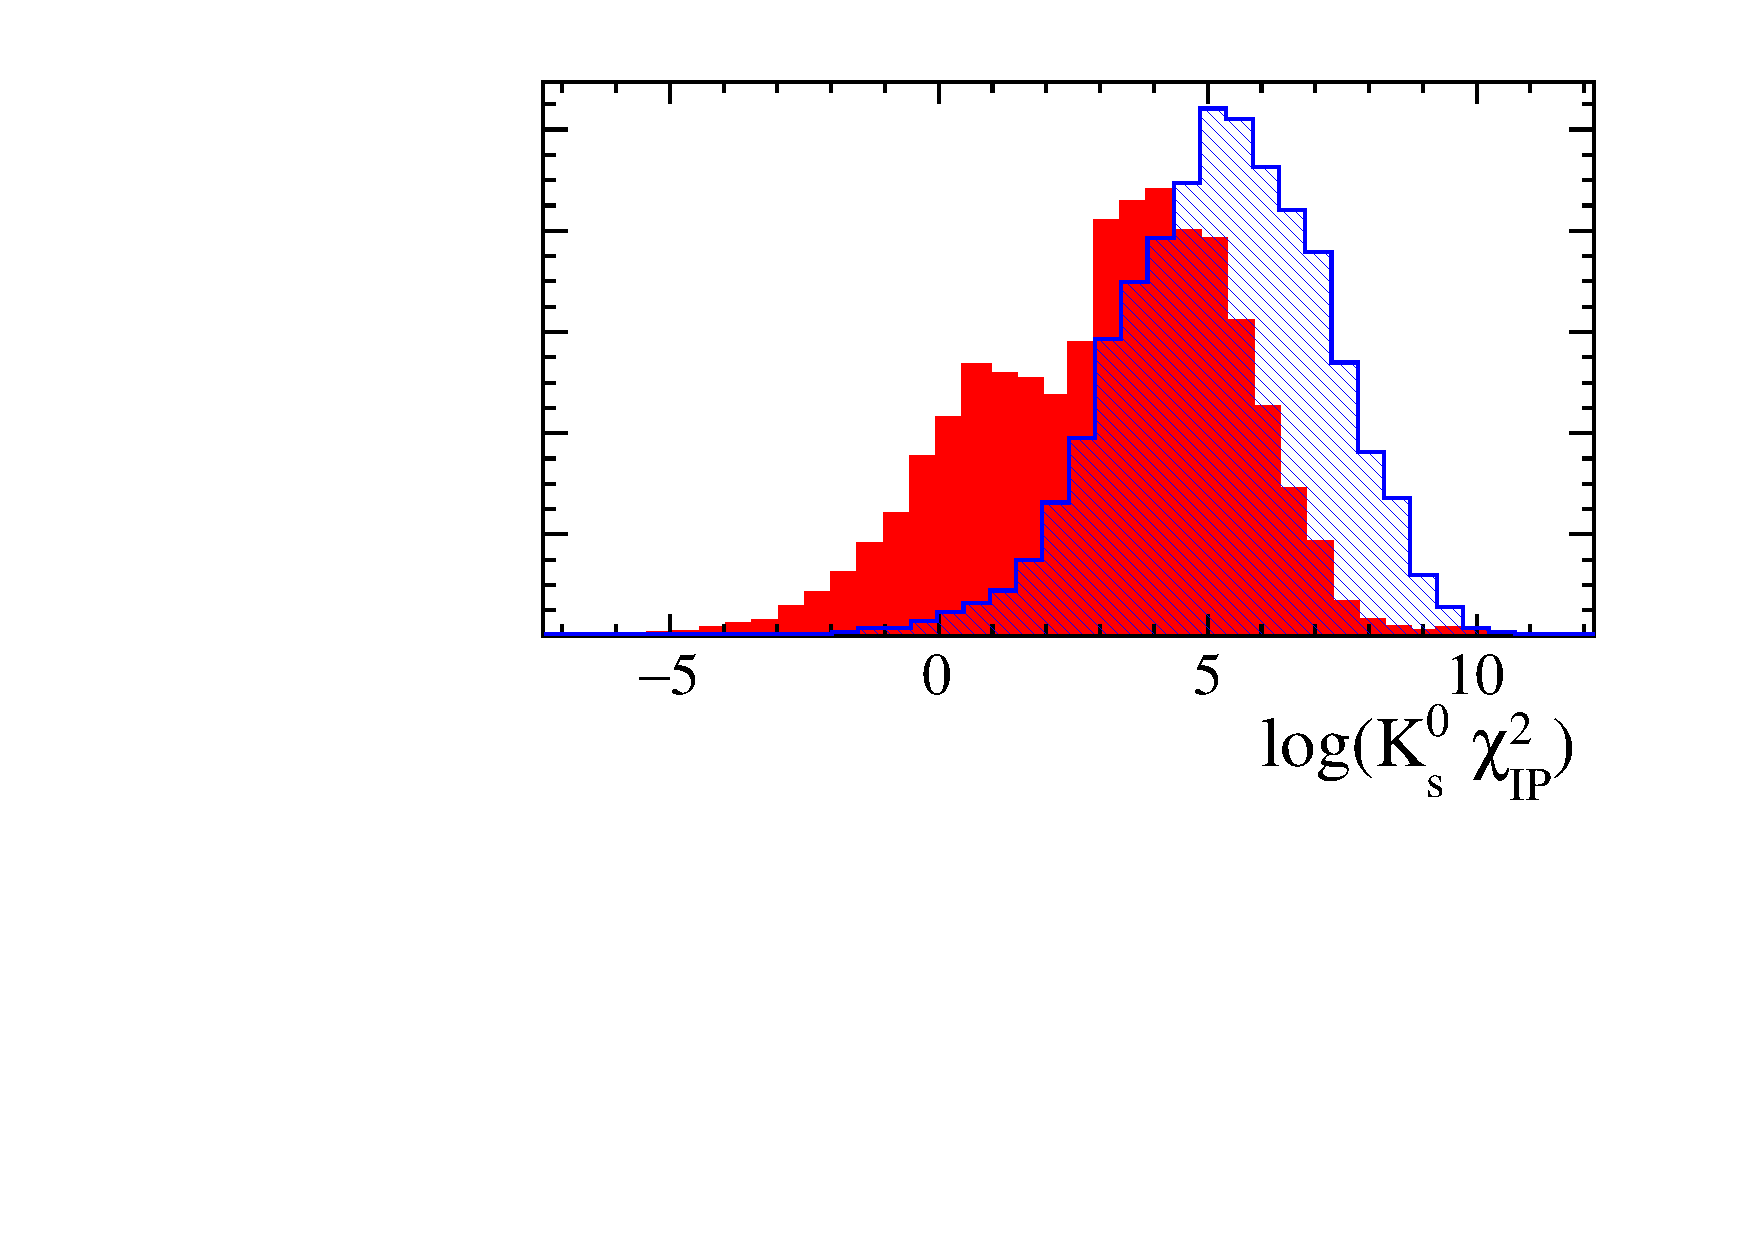
\includegraphics[width=0.3\linewidth]{figures/selection/BDTvariables/BDT_Var_KPiPiPi_LL_log_Ks_IPCHI2_OWNPV_.pdf}
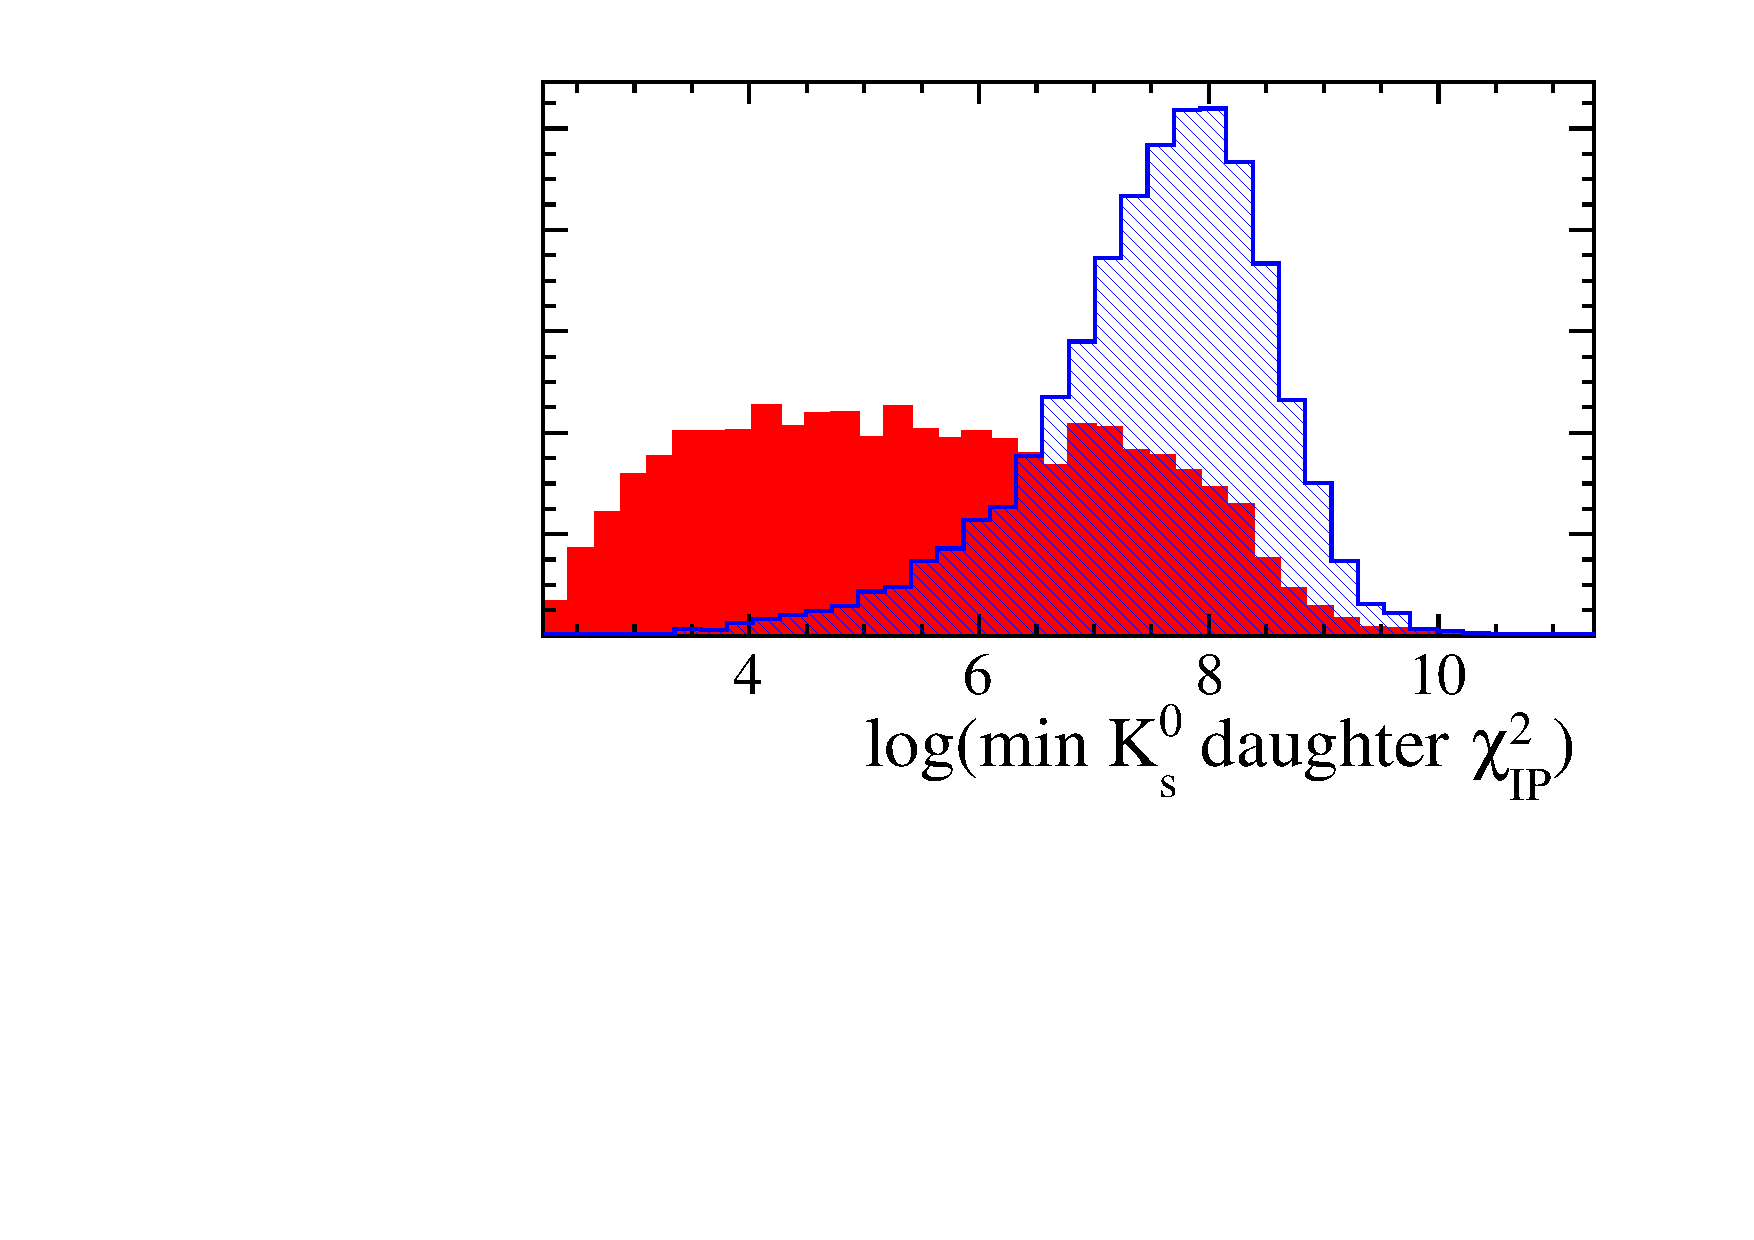
\includegraphics[width=0.3\linewidth]{figures/selection/BDTvariables/BDT_Var_KPiPiPi_LL_log_max_Ksh_IPCHI2_OWNPV_.pdf}
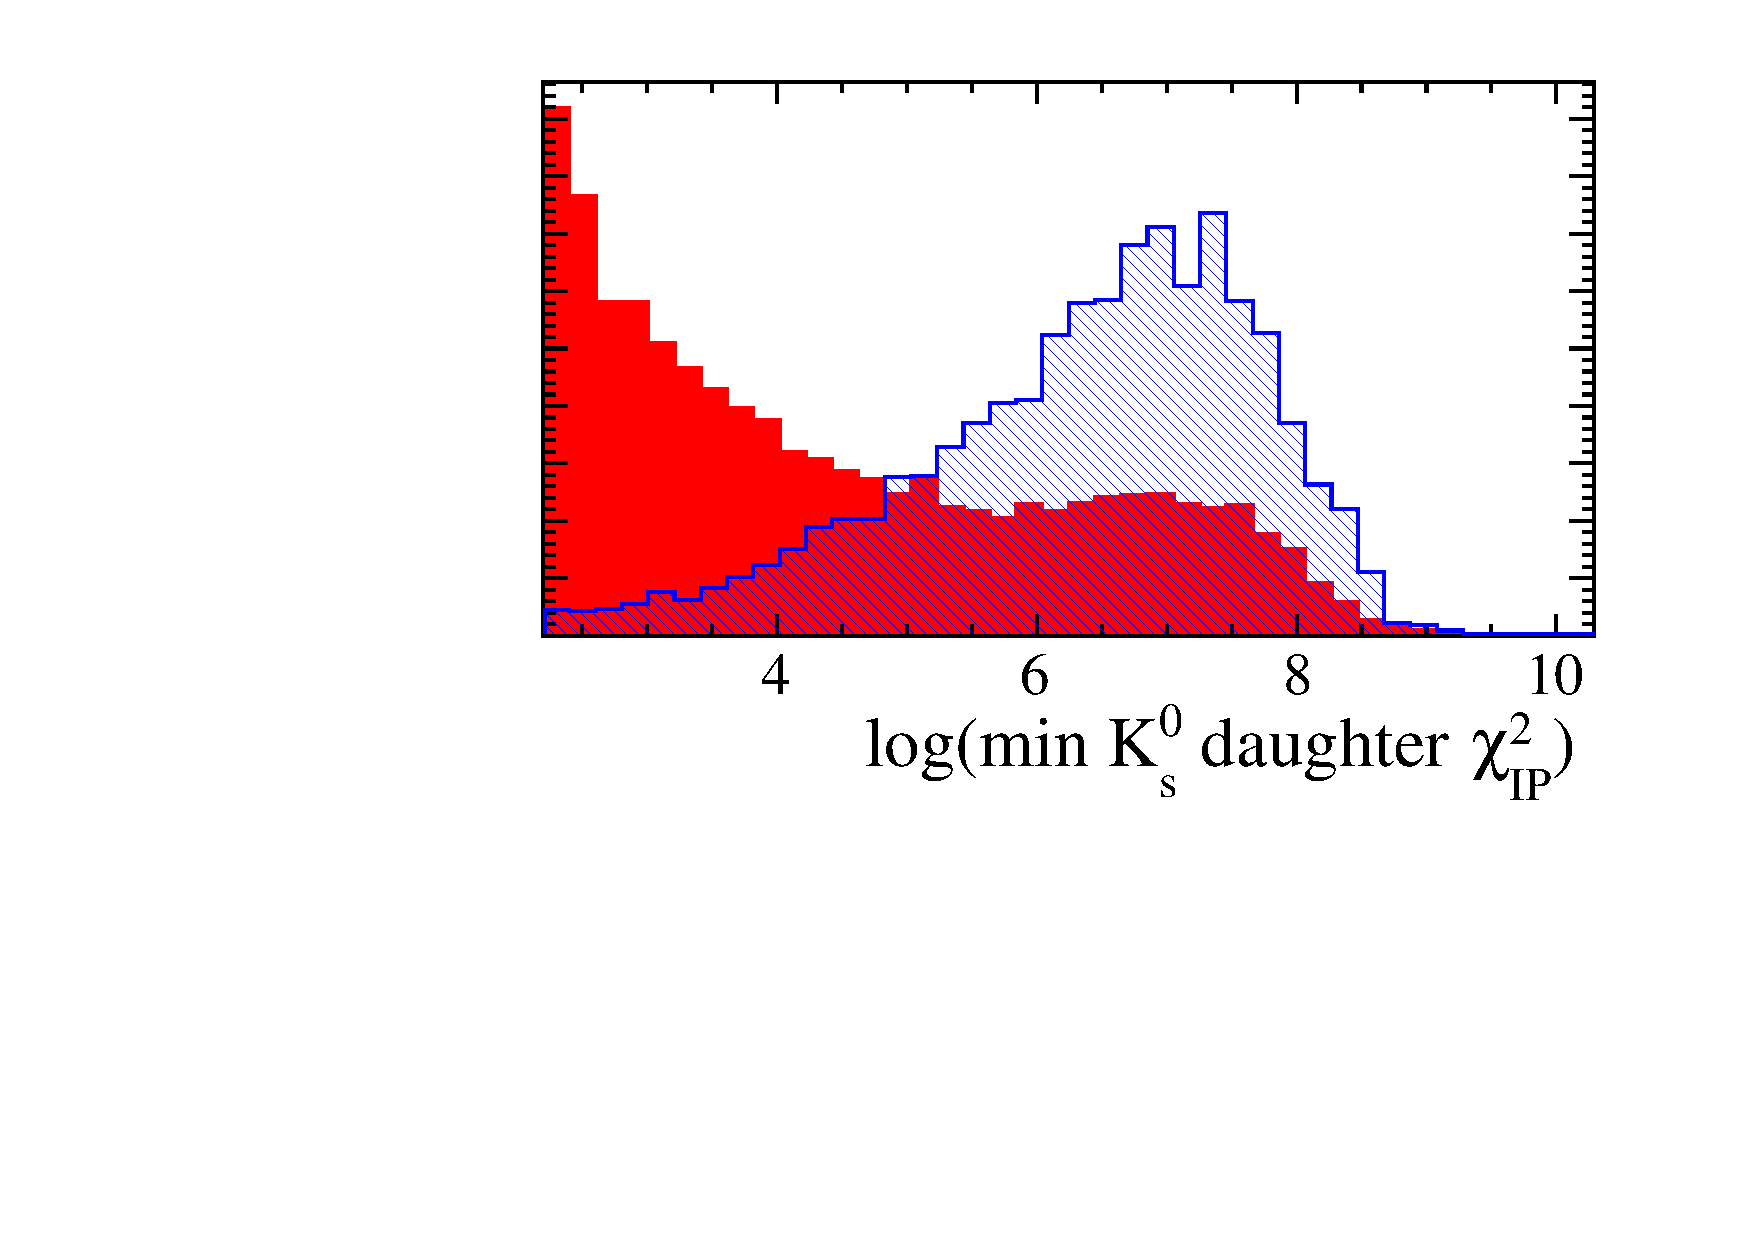
\includegraphics[width=0.3\linewidth]{figures/selection/BDTvariables/BDT_Var_KPiPiPi_LL_log_min_Ksh_IPCHI2_OWNPV_.pdf}
\hfill
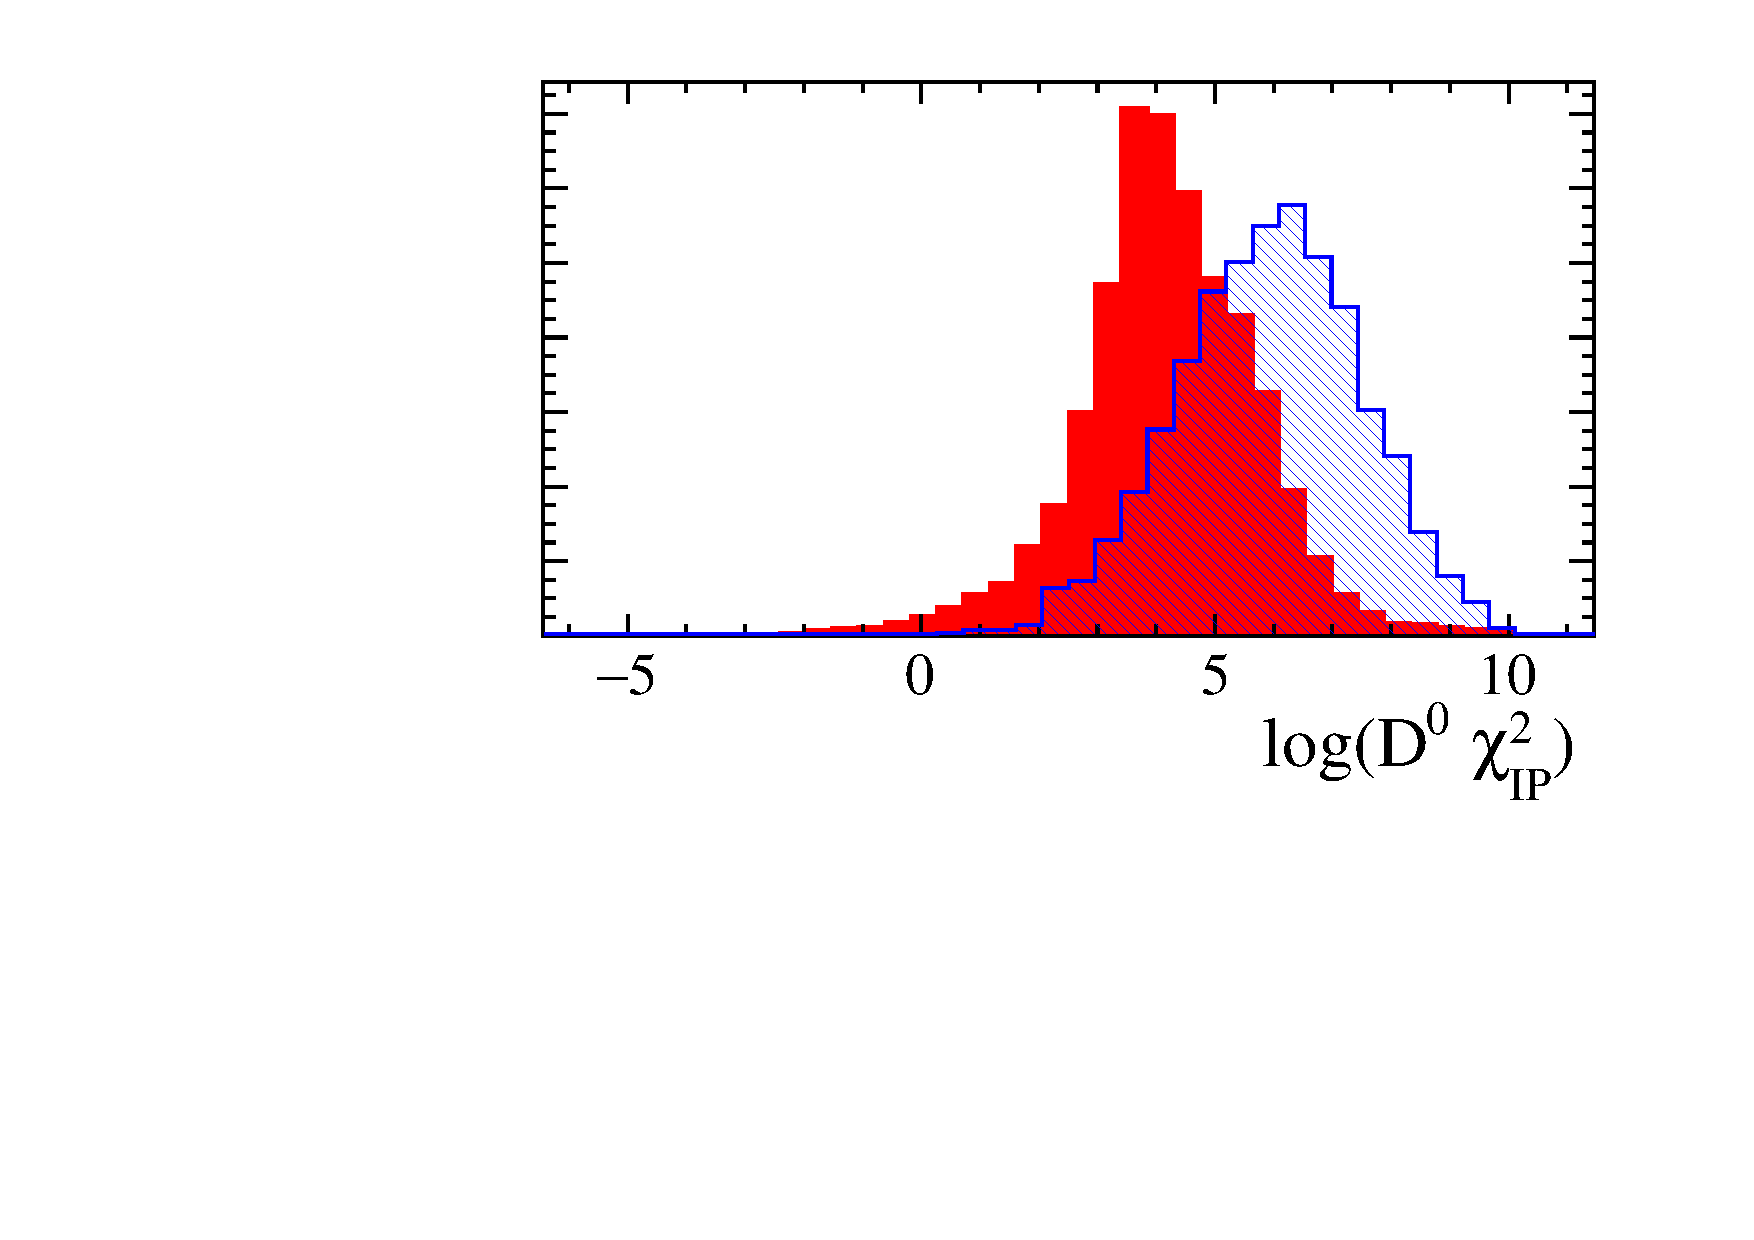
\includegraphics[width=0.3\linewidth]{figures/selection/BDTvariables/BDT_Var_KPiPiPi_LL_log_D0_IPCHI2_OWNPV_.pdf}
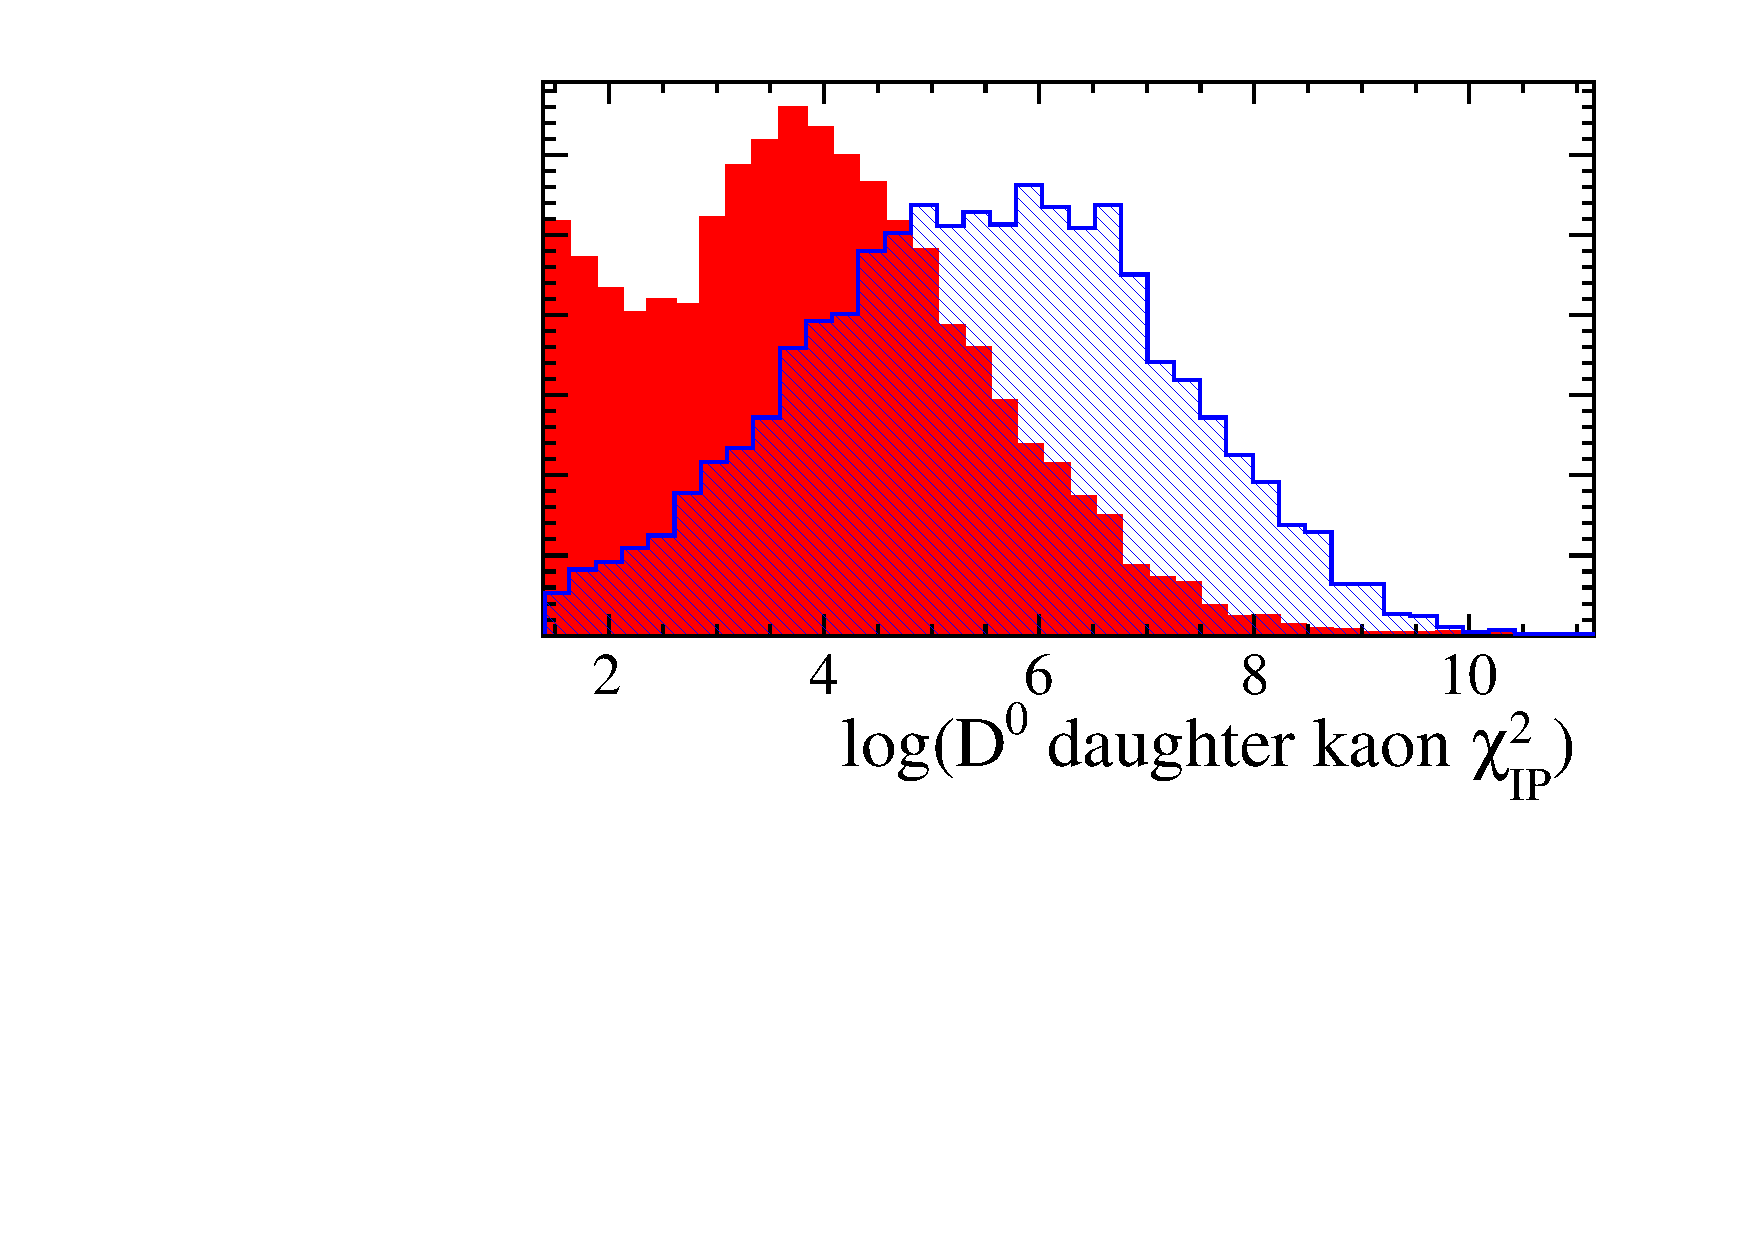
\includegraphics[width=0.3\linewidth]{figures/selection/BDTvariables/BDT_Var_KPiPiPi_LL_log_Dh1_IPCHI2_OWNPV_.pdf}
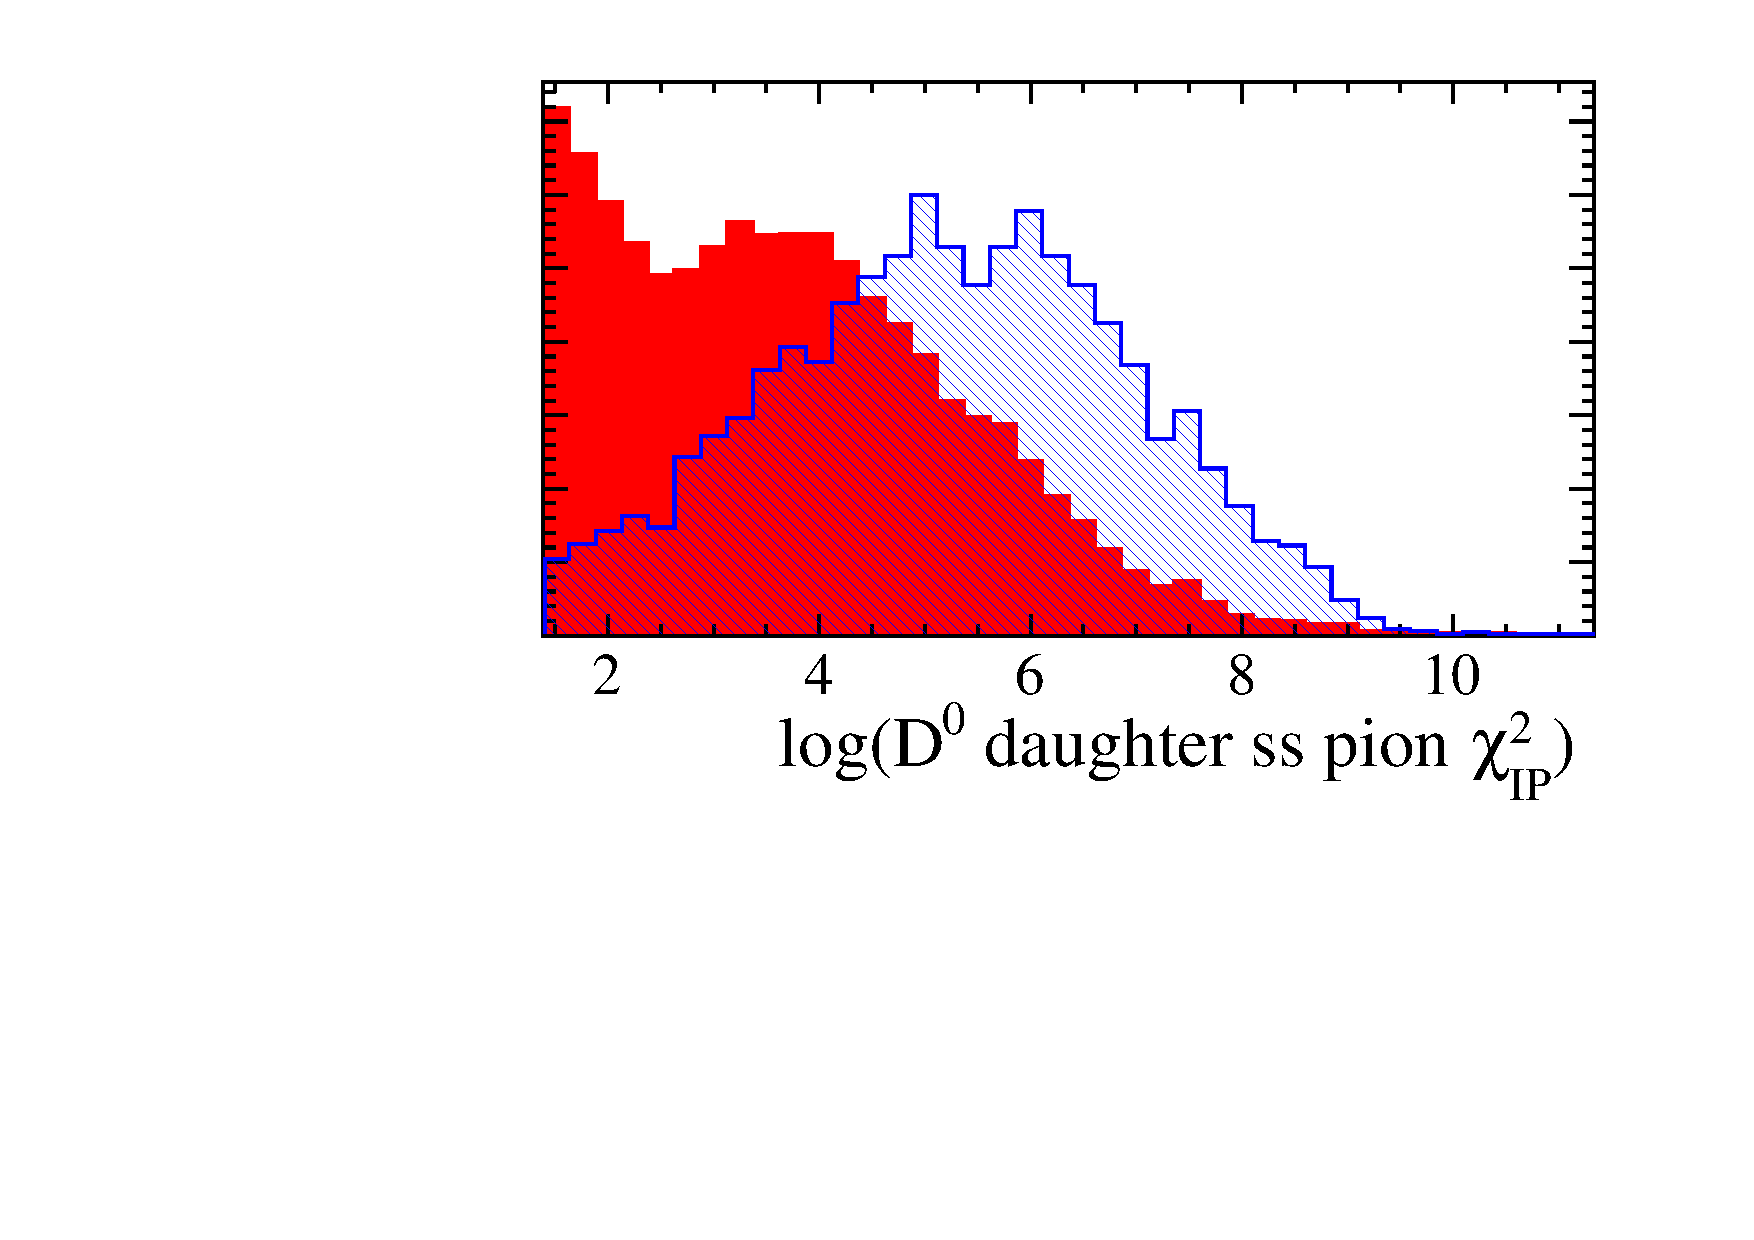
\includegraphics[width=0.3\linewidth]{figures/selection/BDTvariables/BDT_Var_KPiPiPi_LL_log_Dhss_IPCHI2_OWNPV_.pdf}
\hfill
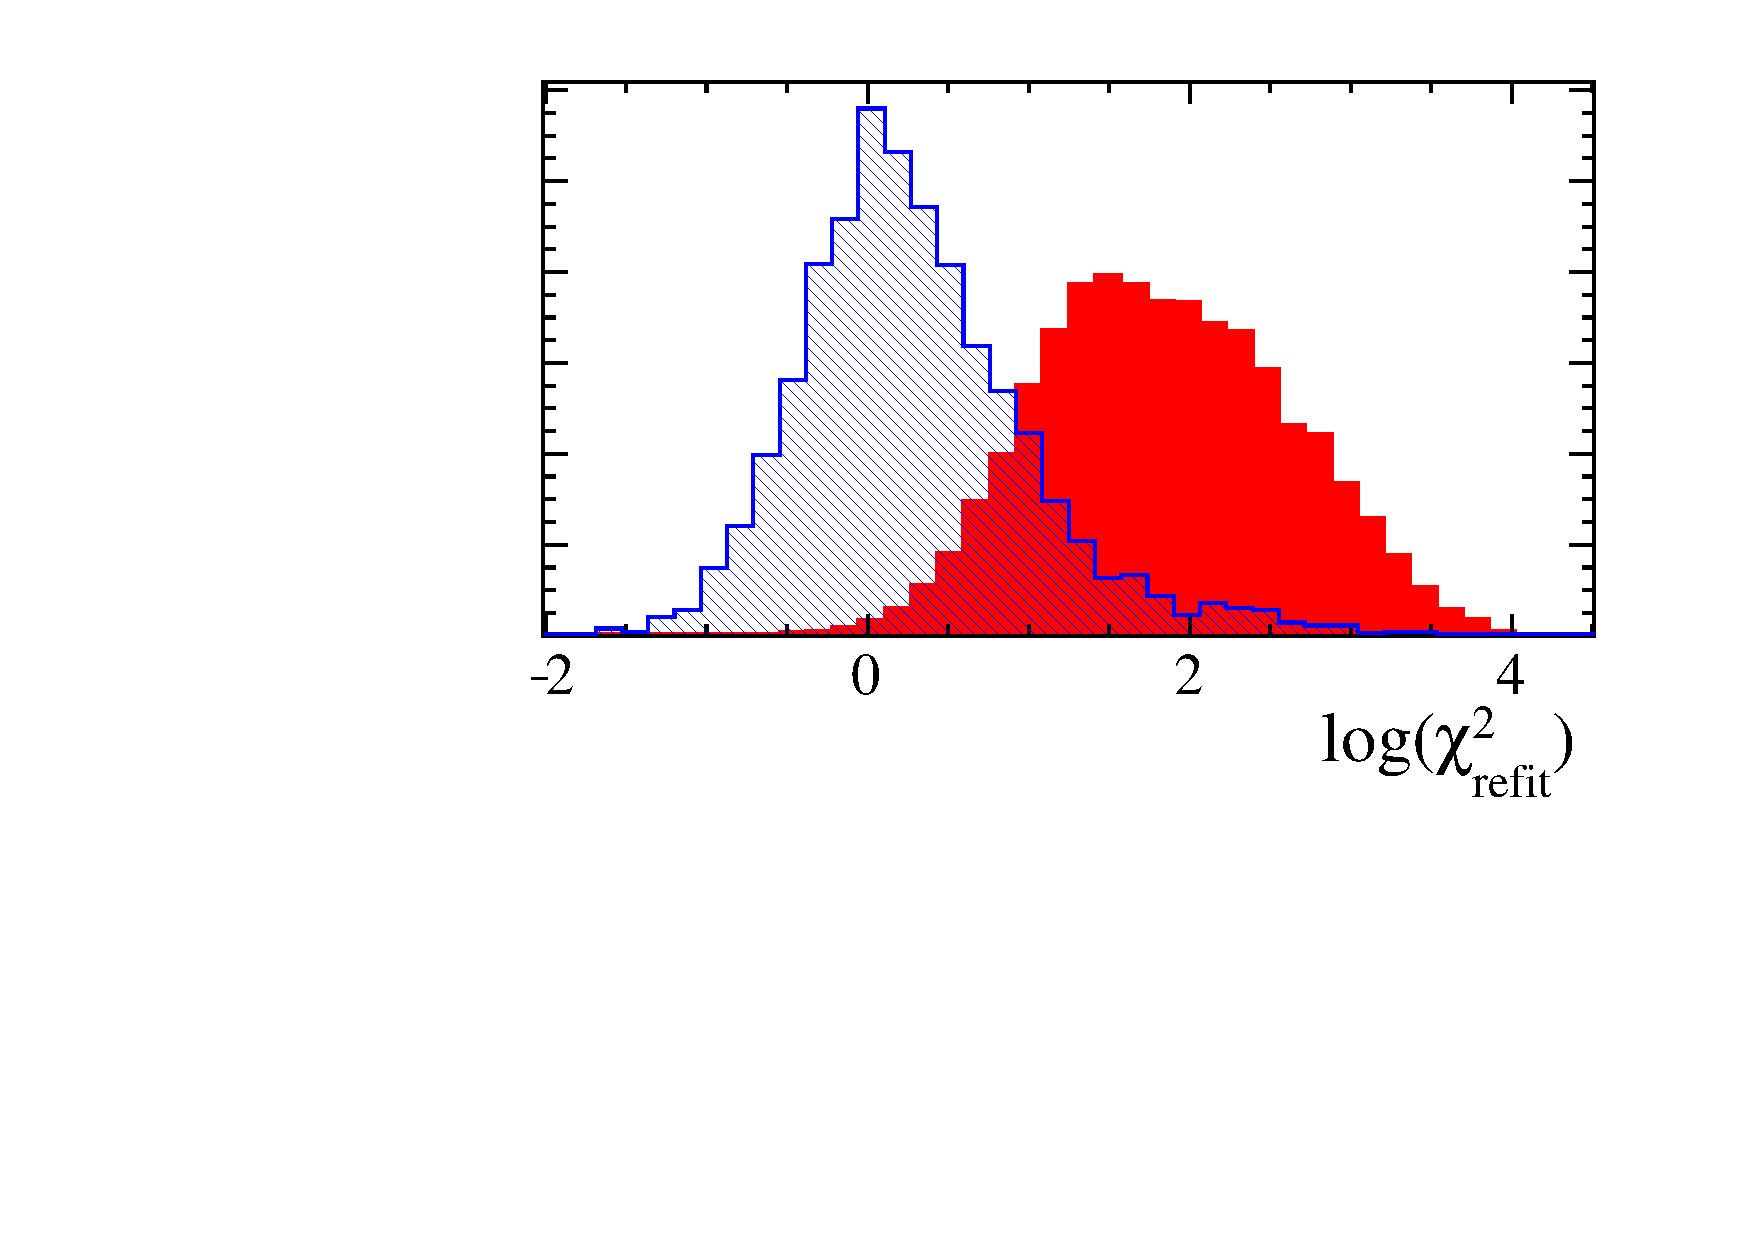
\includegraphics[width=0.3\linewidth]{figures/selection/BDTvariables/BDT_Var_KPiPiPi_LL_log_Bu_D0constKS0constPVconst_CHI2NDOF_.pdf}
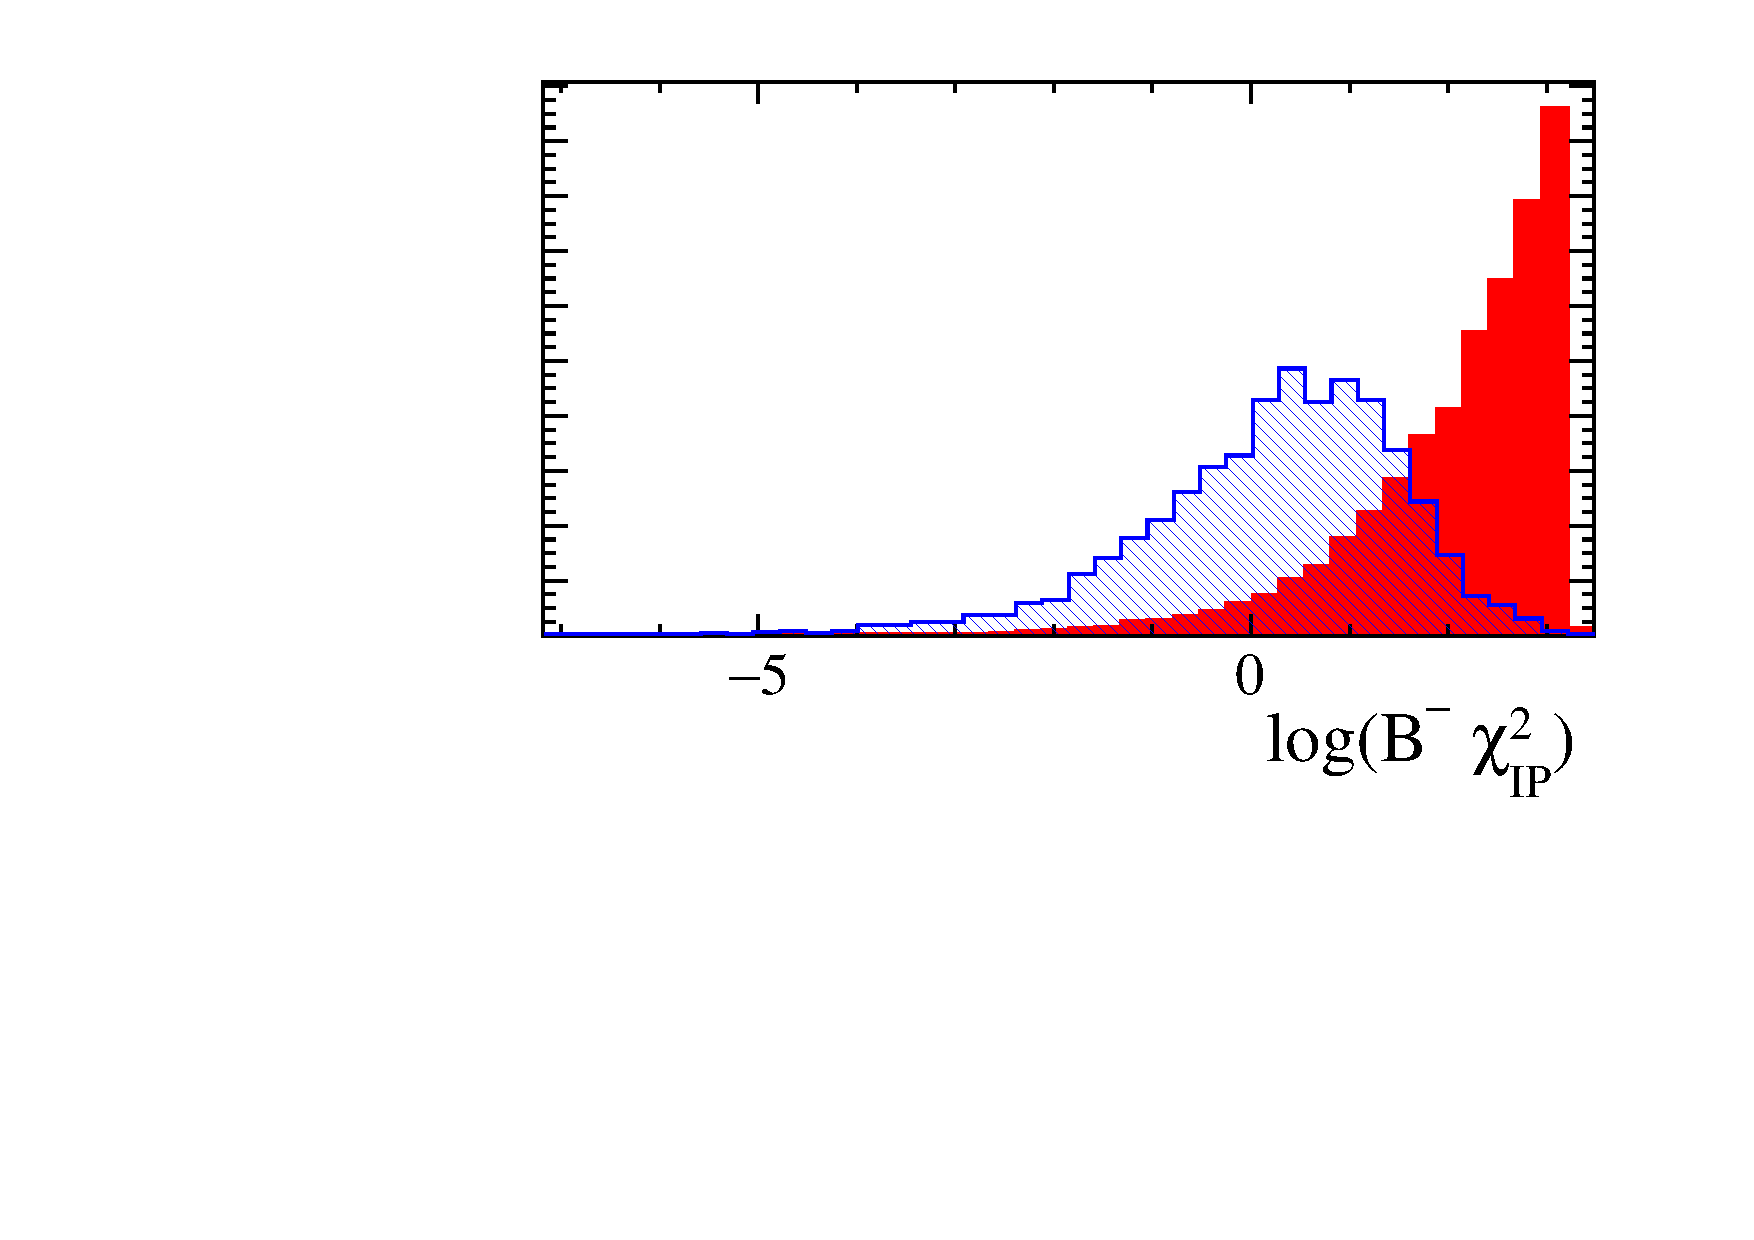
\includegraphics[width=0.3\linewidth]{figures/selection/BDTvariables/BDT_Var_KPiPiPi_LL_log_Bu_IPCHI2_OWNPV_.pdf}
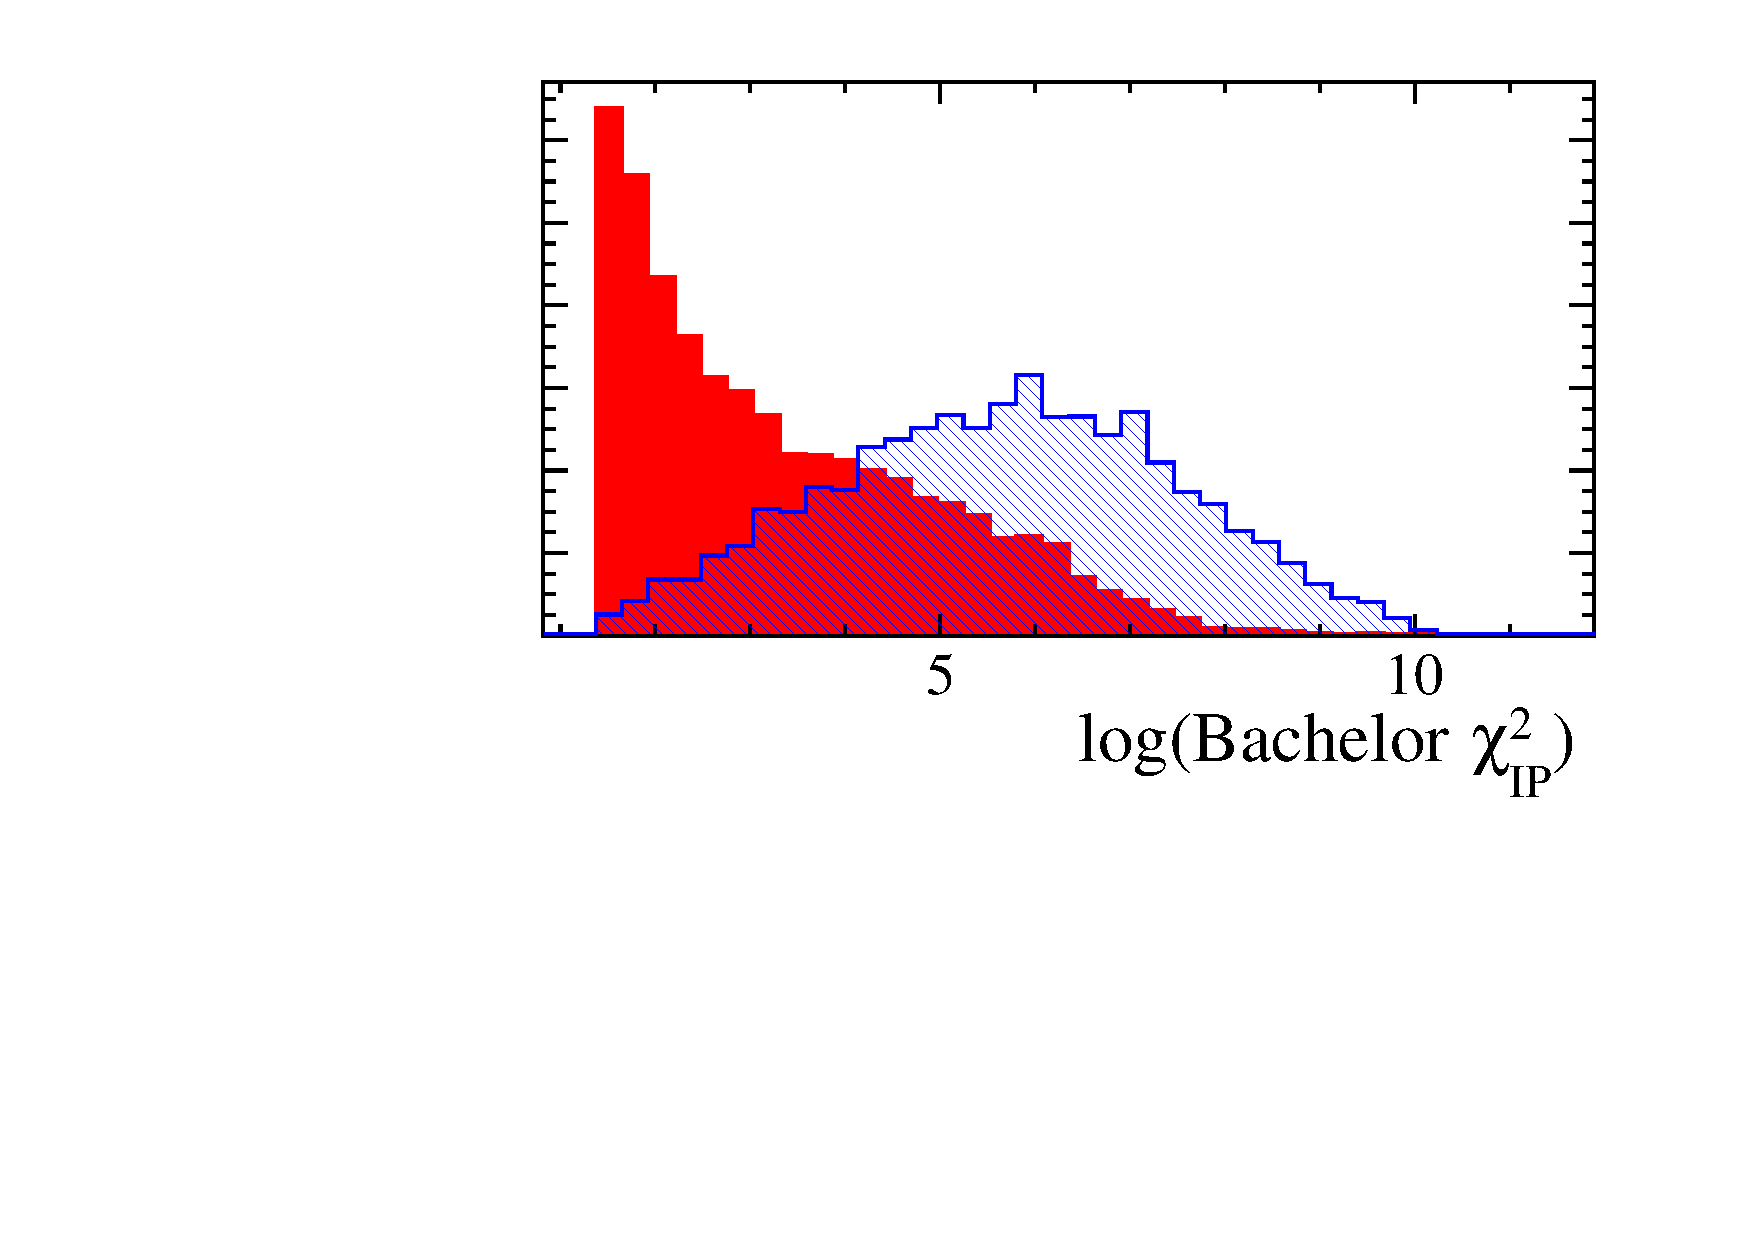
\includegraphics[width=0.3\linewidth]{figures/selection/BDTvariables/BDT_Var_KPiPiPi_LL_log_Bach_IPCHI2_OWNPV_.pdf}
\hfill
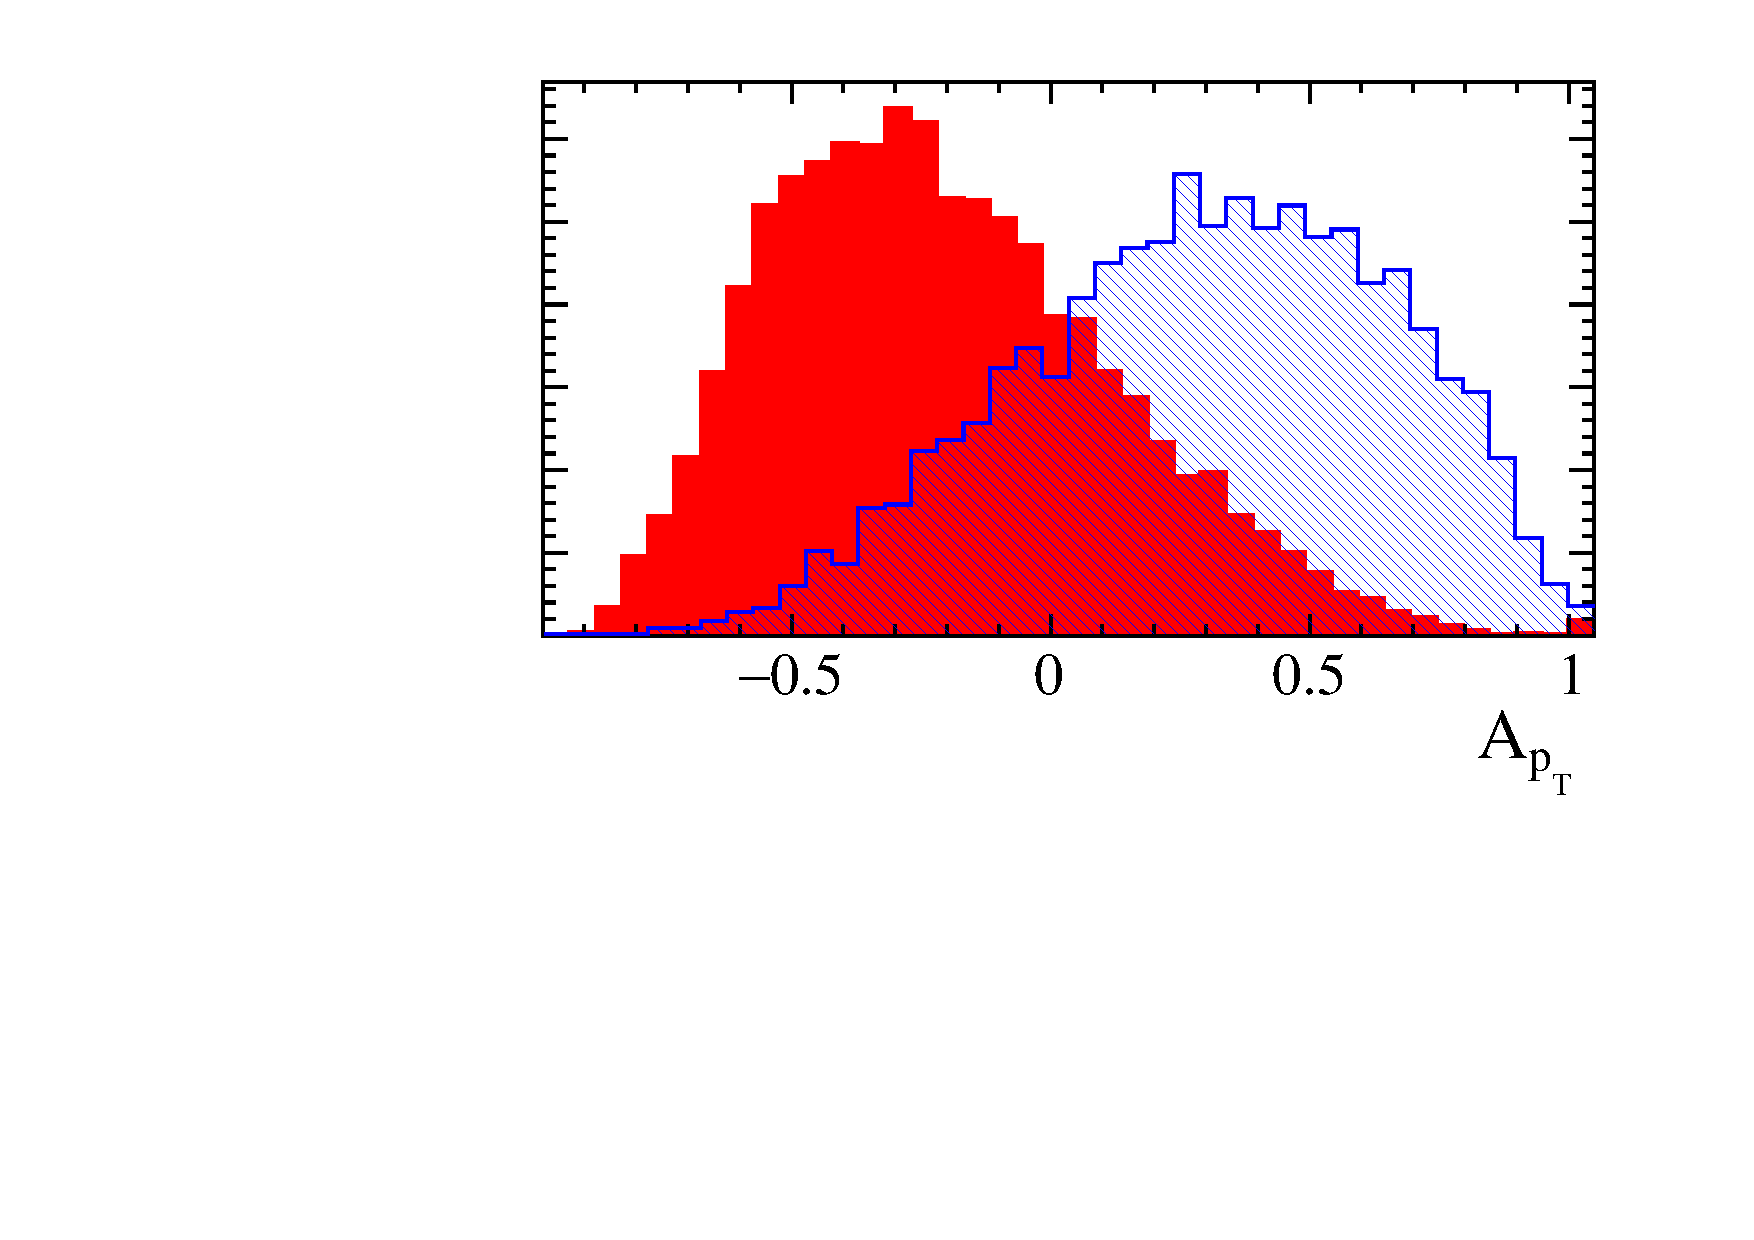
\includegraphics[width=0.3\linewidth]{{figures/selection/BDTvariables/BDT_Var_KPiPiPi_LL_Bu_ptasy_1.50}.pdf}
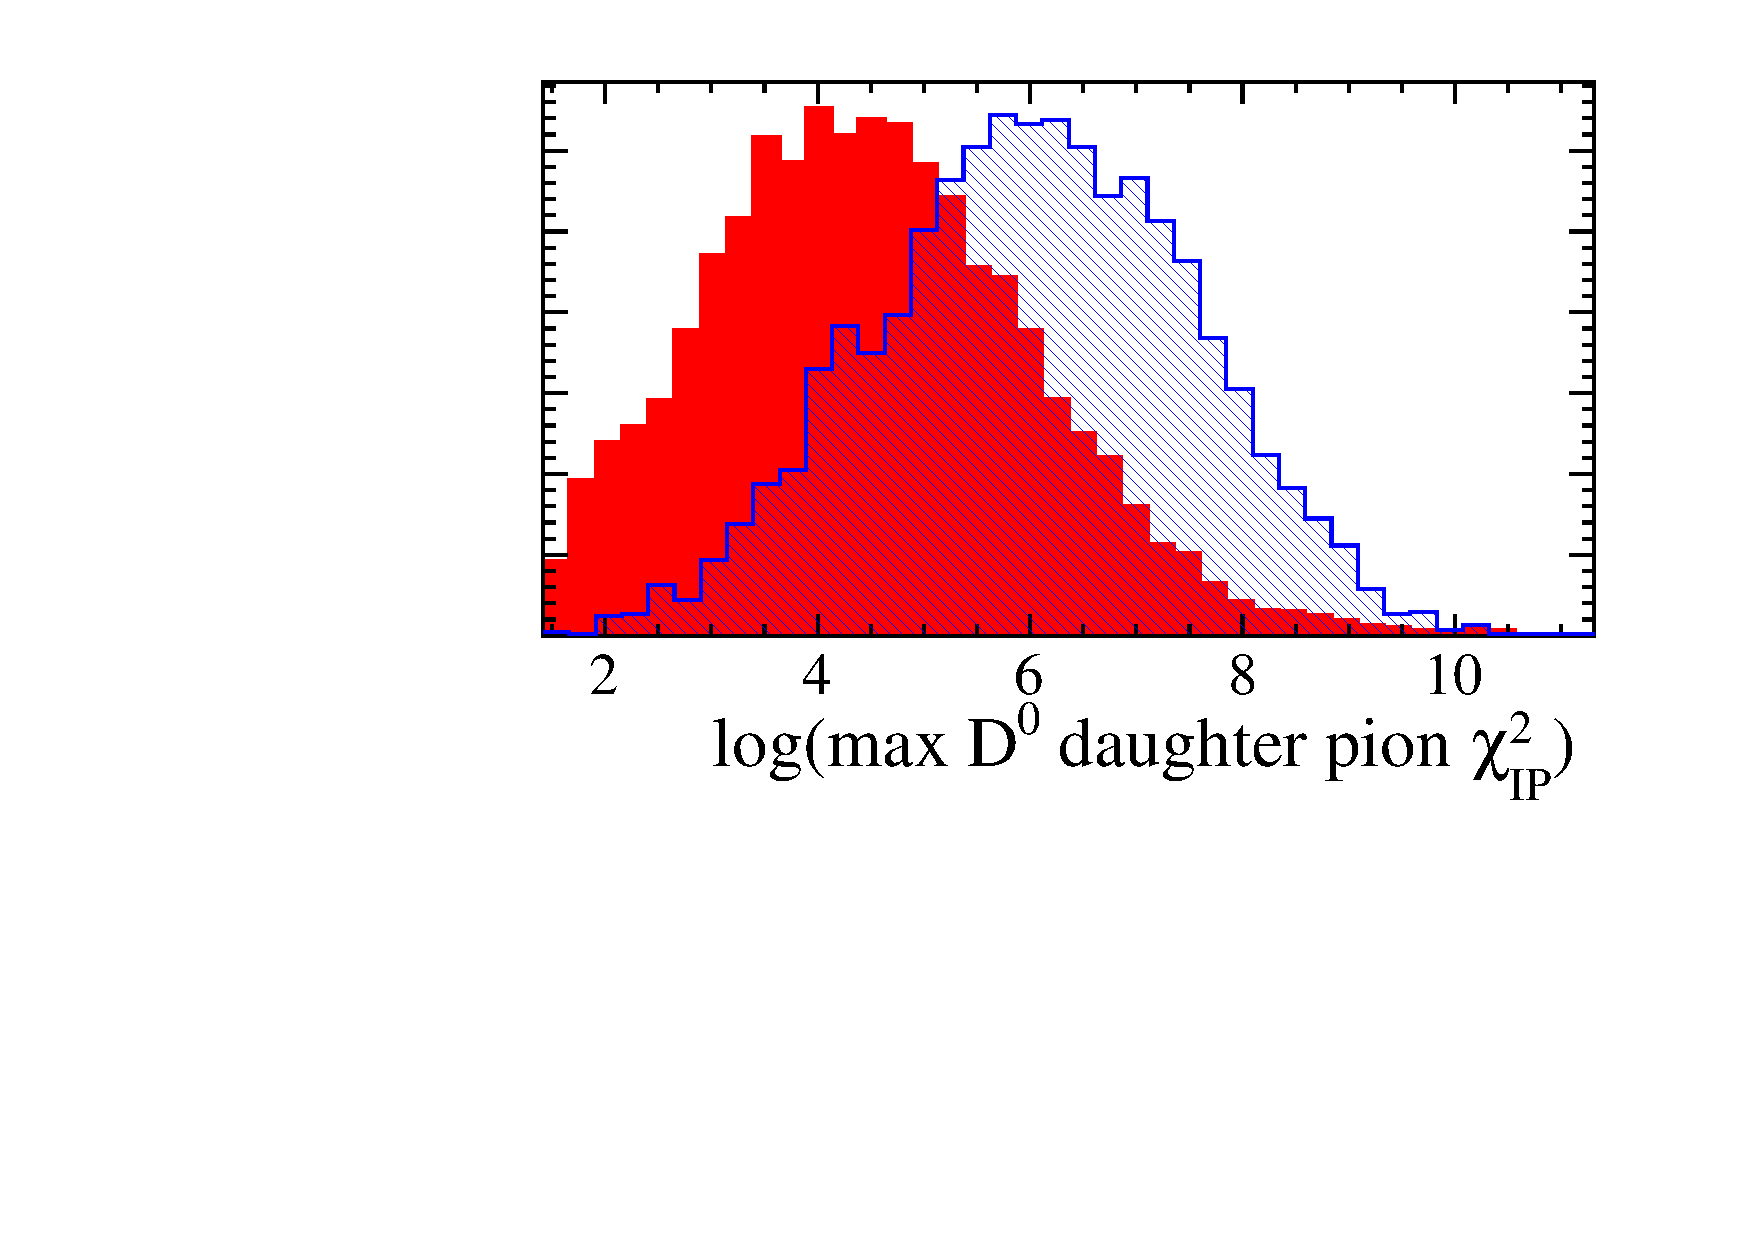
\includegraphics[width=0.3\linewidth]{figures/selection/BDTvariables/BDT_Var_KPiPiPi_LL_log_max_Dh_IPCHI2_OWNPV_.pdf}
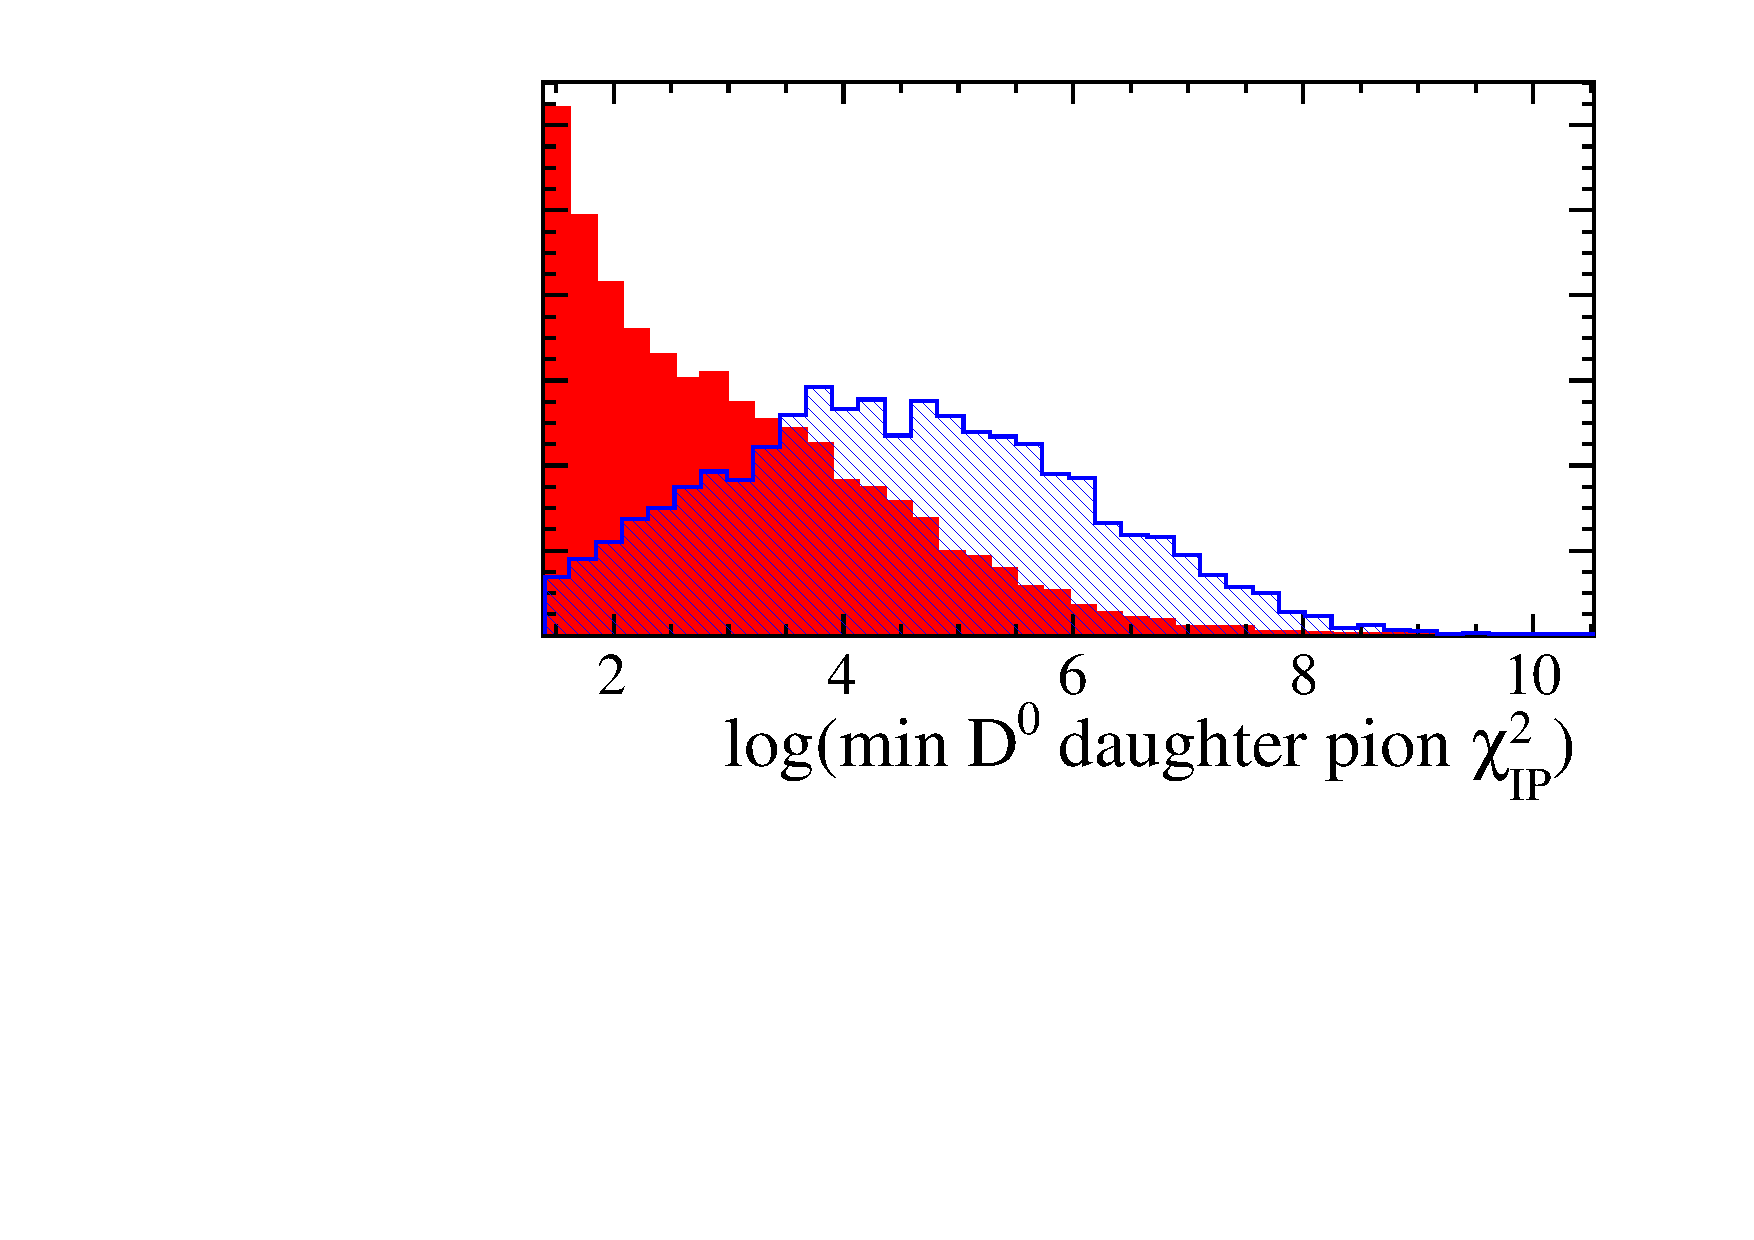
\includegraphics[width=0.3\linewidth]{figures/selection/BDTvariables/BDT_Var_KPiPiPi_LL_log_min_Dh_IPCHI2_OWNPV_.pdf}
\caption{Distributions of the input variables using the signal (blue) and background (red) training samples for the four-body LL BDT. The variable $A_{\pt}$ represents the \pt asymmetry as defined in \eqn~\ref{ptasy} and ``max (min) \KS daughter \chisqip'' refers to the \chisqip of the \KS daughter which has the largest (smallest) \chisqip. The particle name ``D daughter ss'' refers to the pion from the \Dz meson which has the same sign as the kaon. All distributions have been normalised to unity in order to easily compare their shape, therefore the vertical axis is not labelled as it is not of interest here.}
\label{BDTinputdist4bodyLL}
\end{figure}

\begin{figure}
\centering
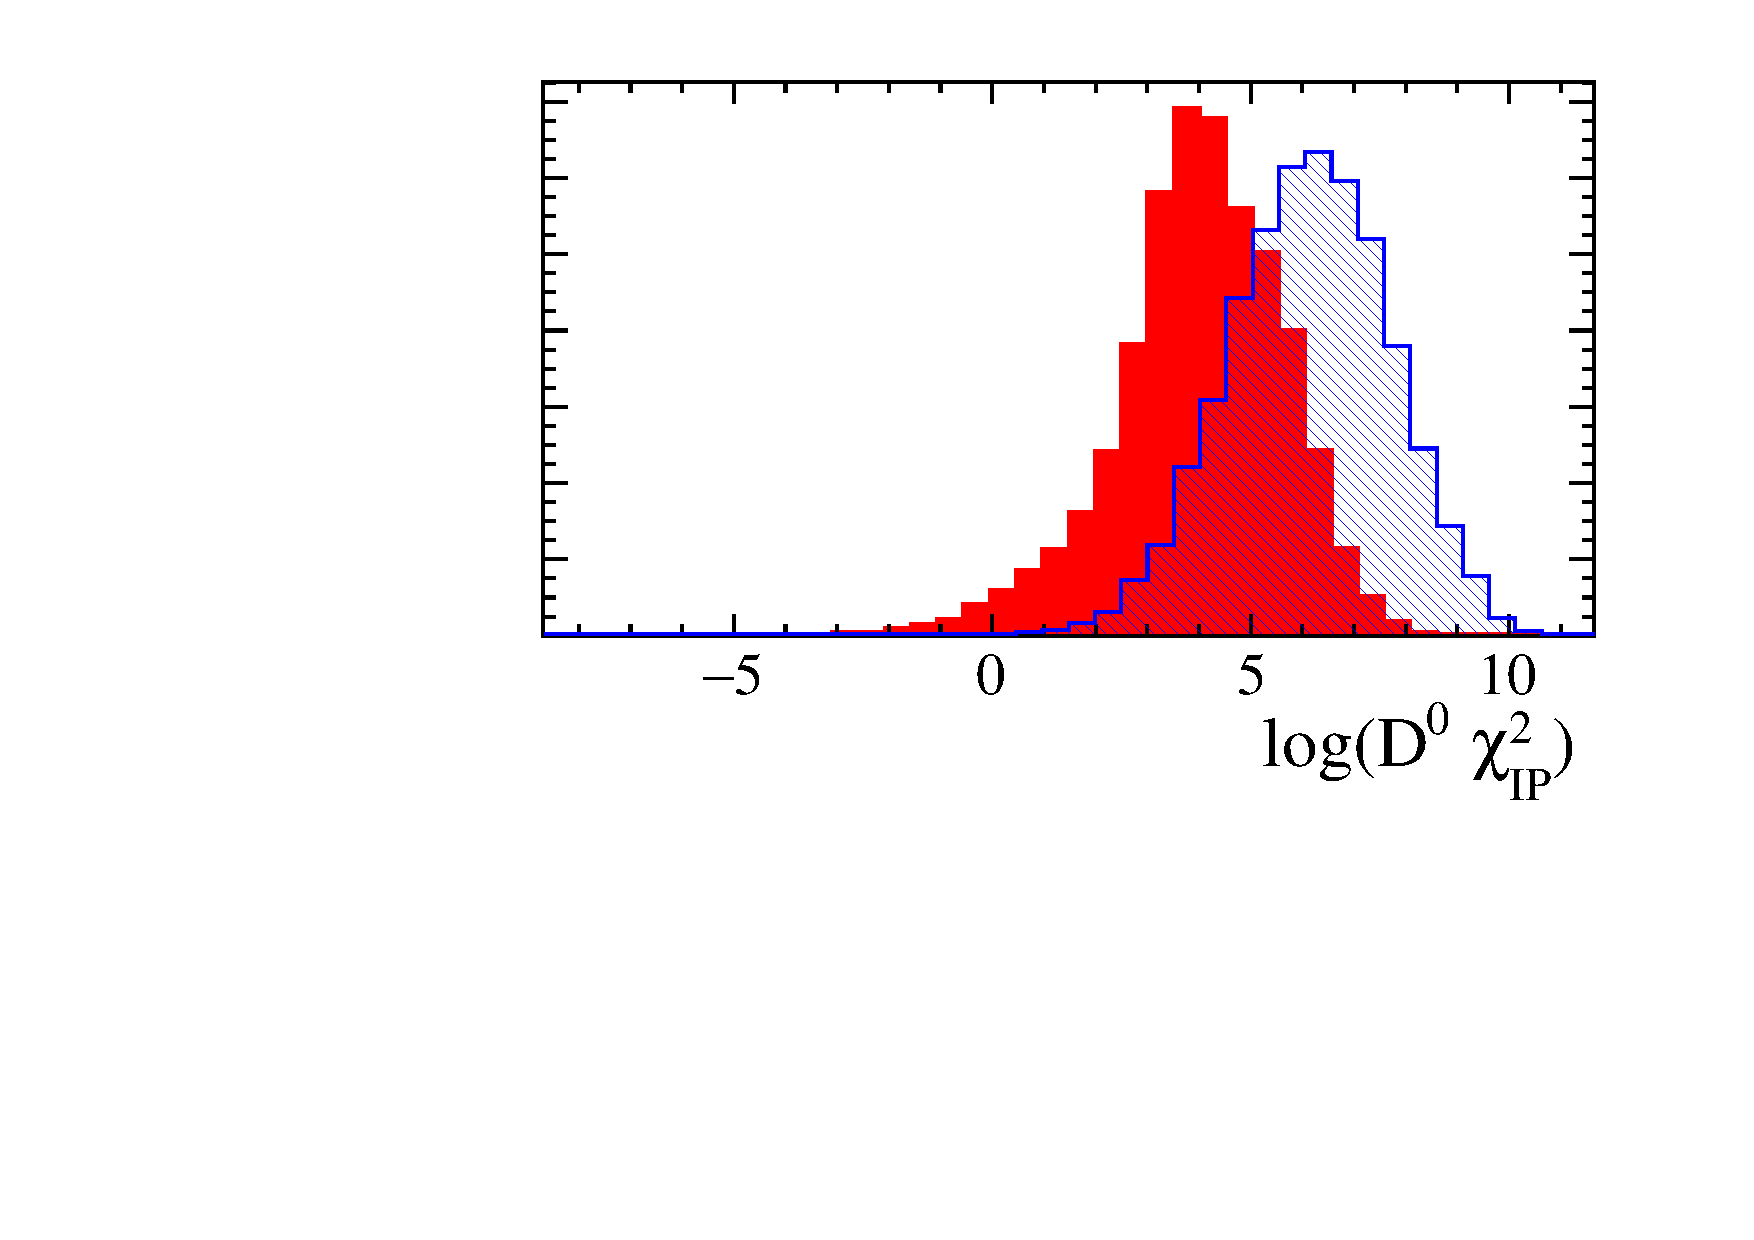
\includegraphics[width=0.3\linewidth]{figures/selection/BDTvariables/BDT_Var_KPiPiPi_DD_log_D0_IPCHI2_OWNPV_.pdf}
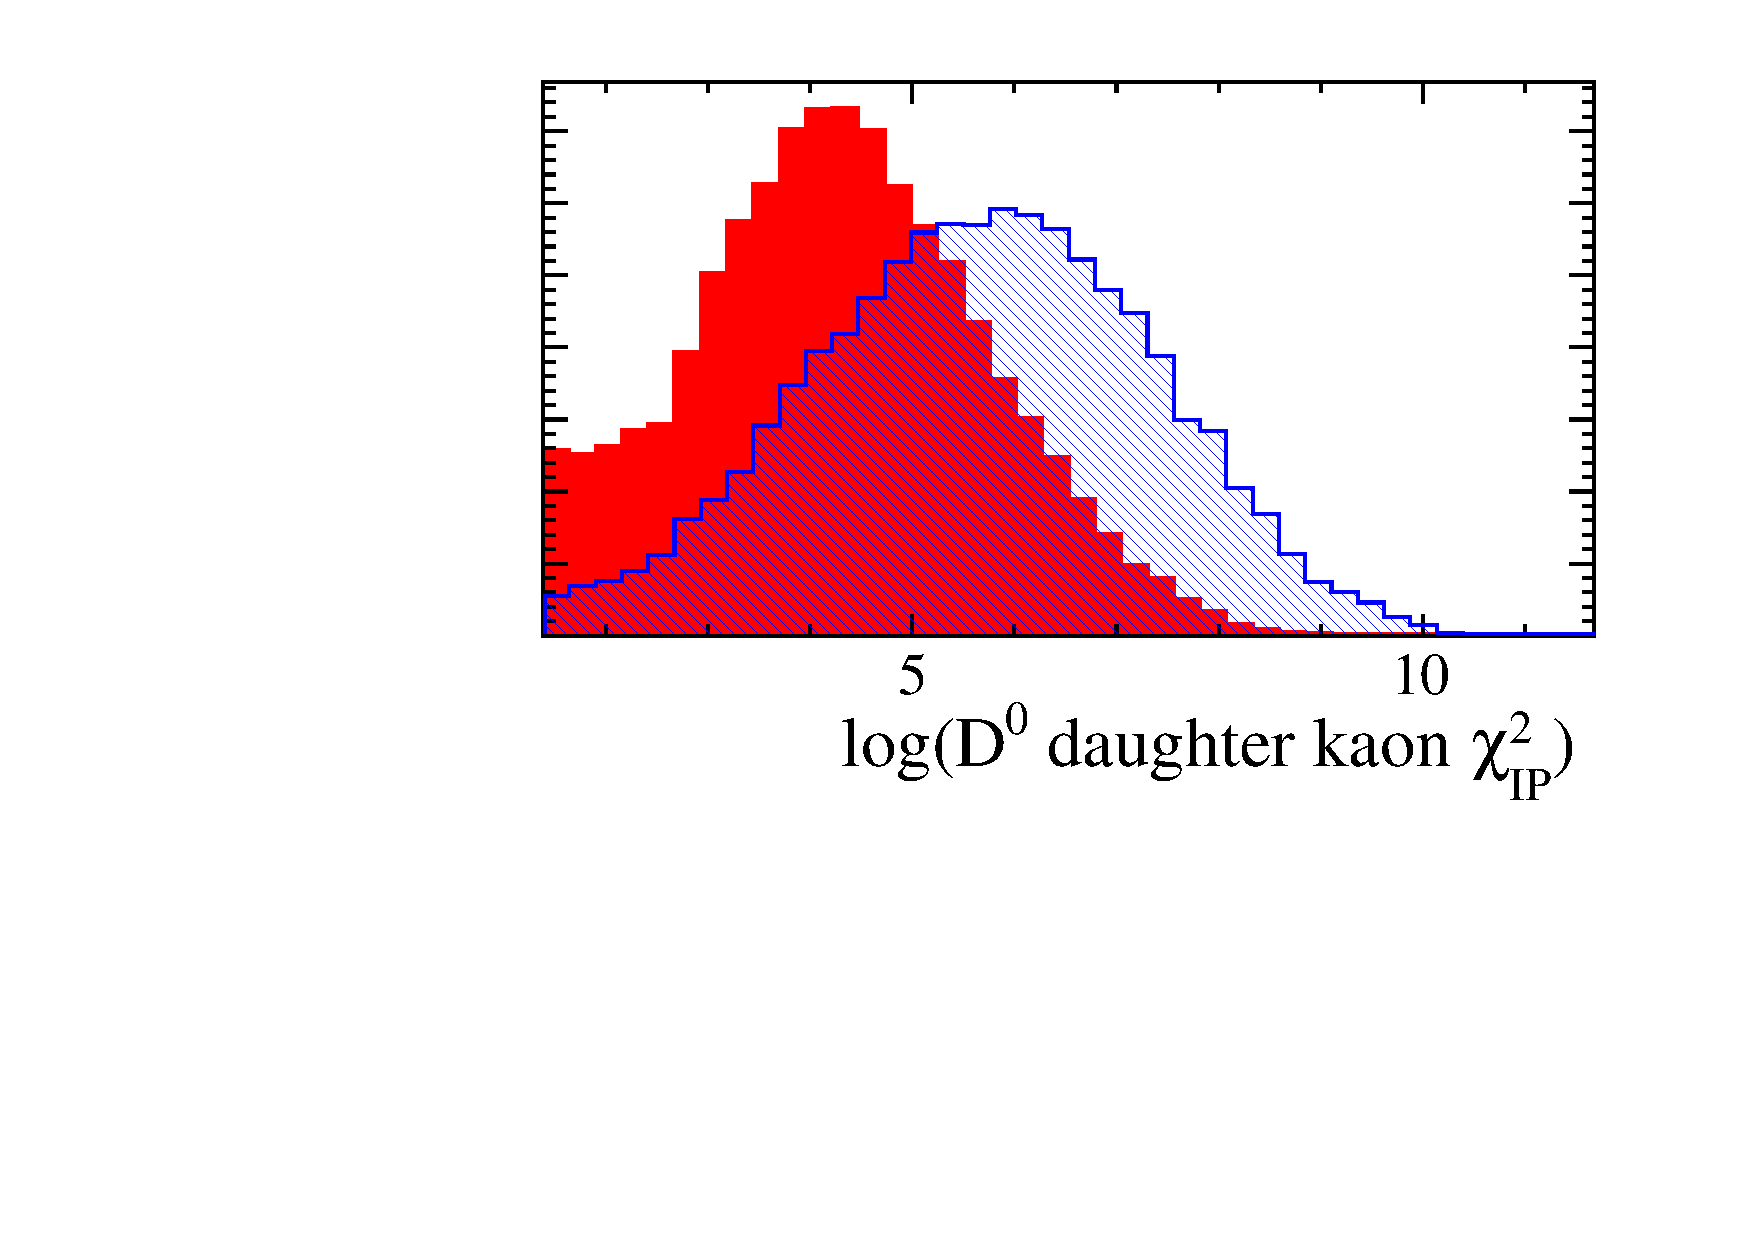
\includegraphics[width=0.3\linewidth]{figures/selection/BDTvariables/BDT_Var_KPiPiPi_DD_log_Dh1_IPCHI2_OWNPV_.pdf}
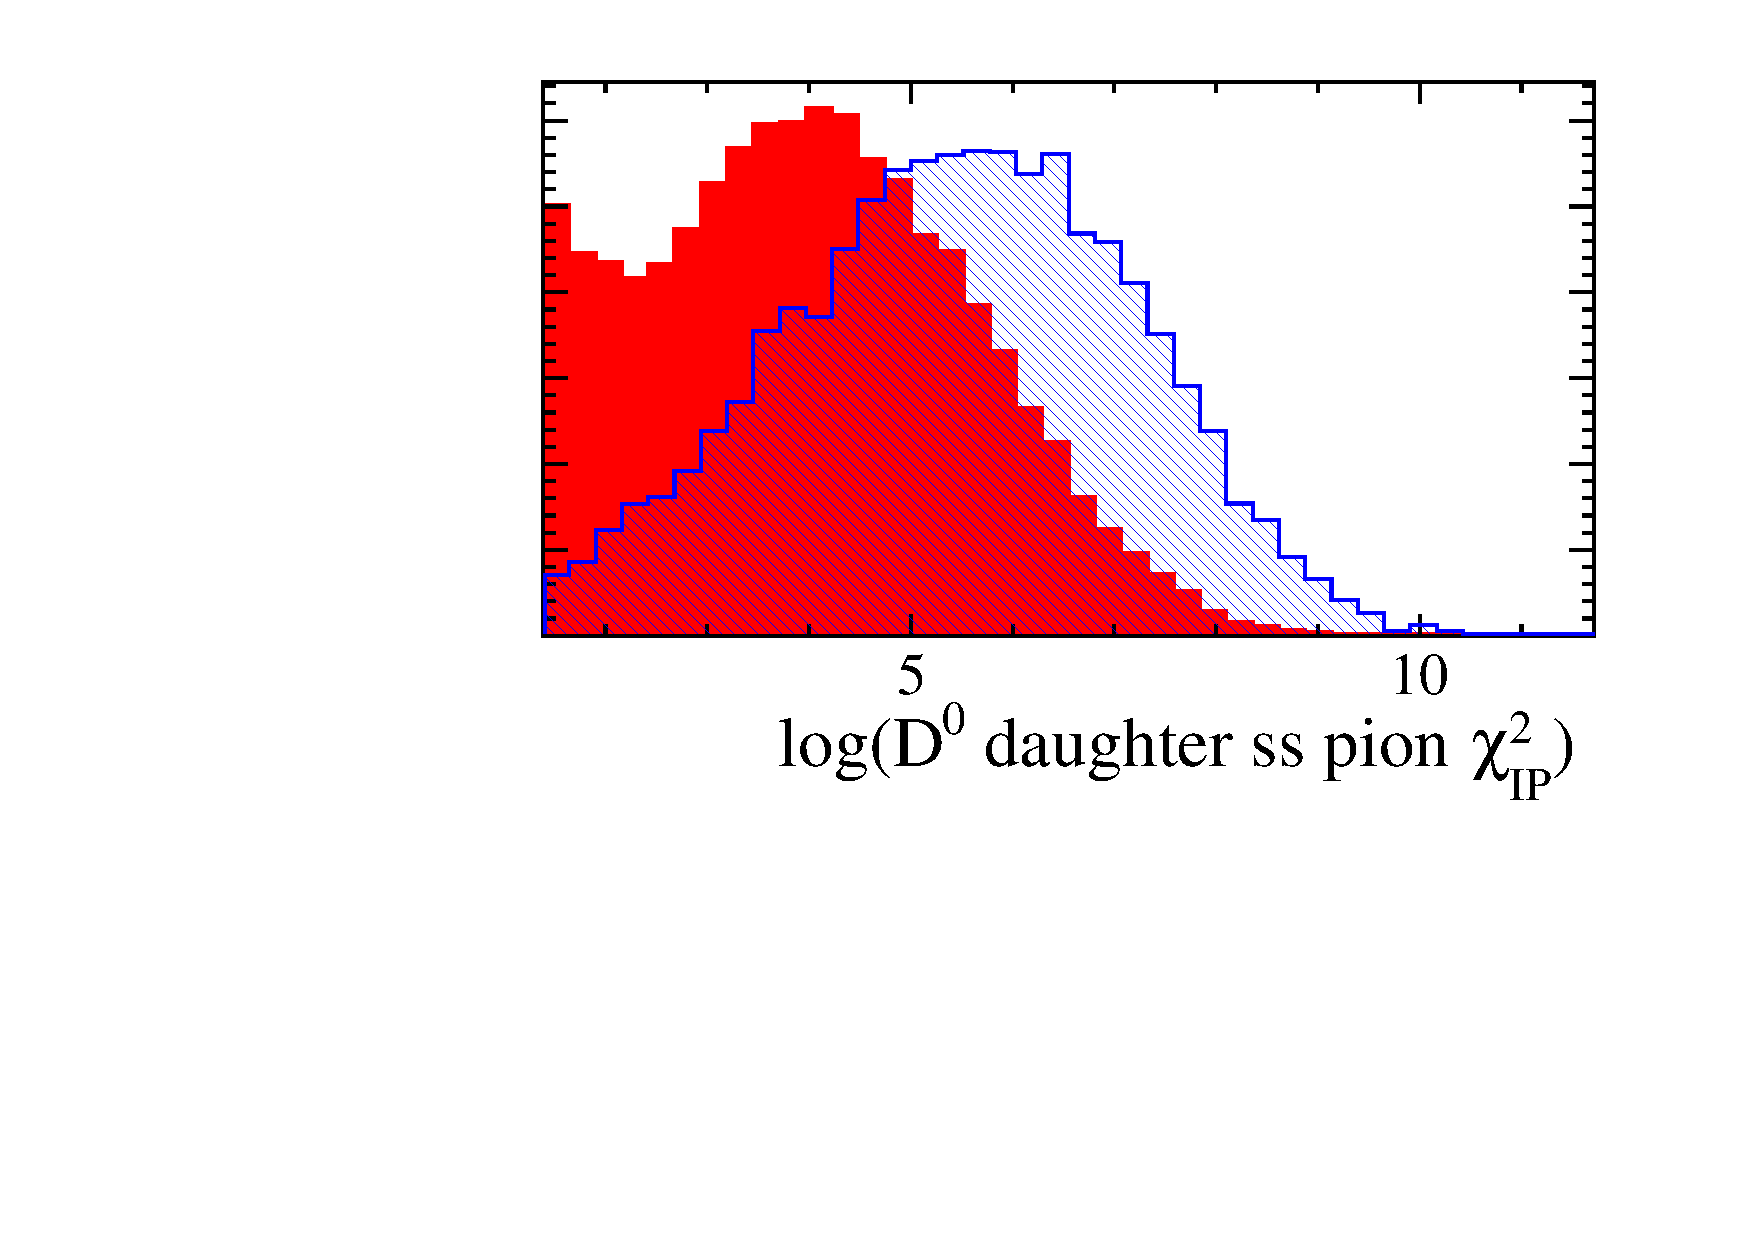
\includegraphics[width=0.3\linewidth]{figures/selection/BDTvariables/BDT_Var_KPiPiPi_DD_log_Dhss_IPCHI2_OWNPV_.pdf}
\hfill
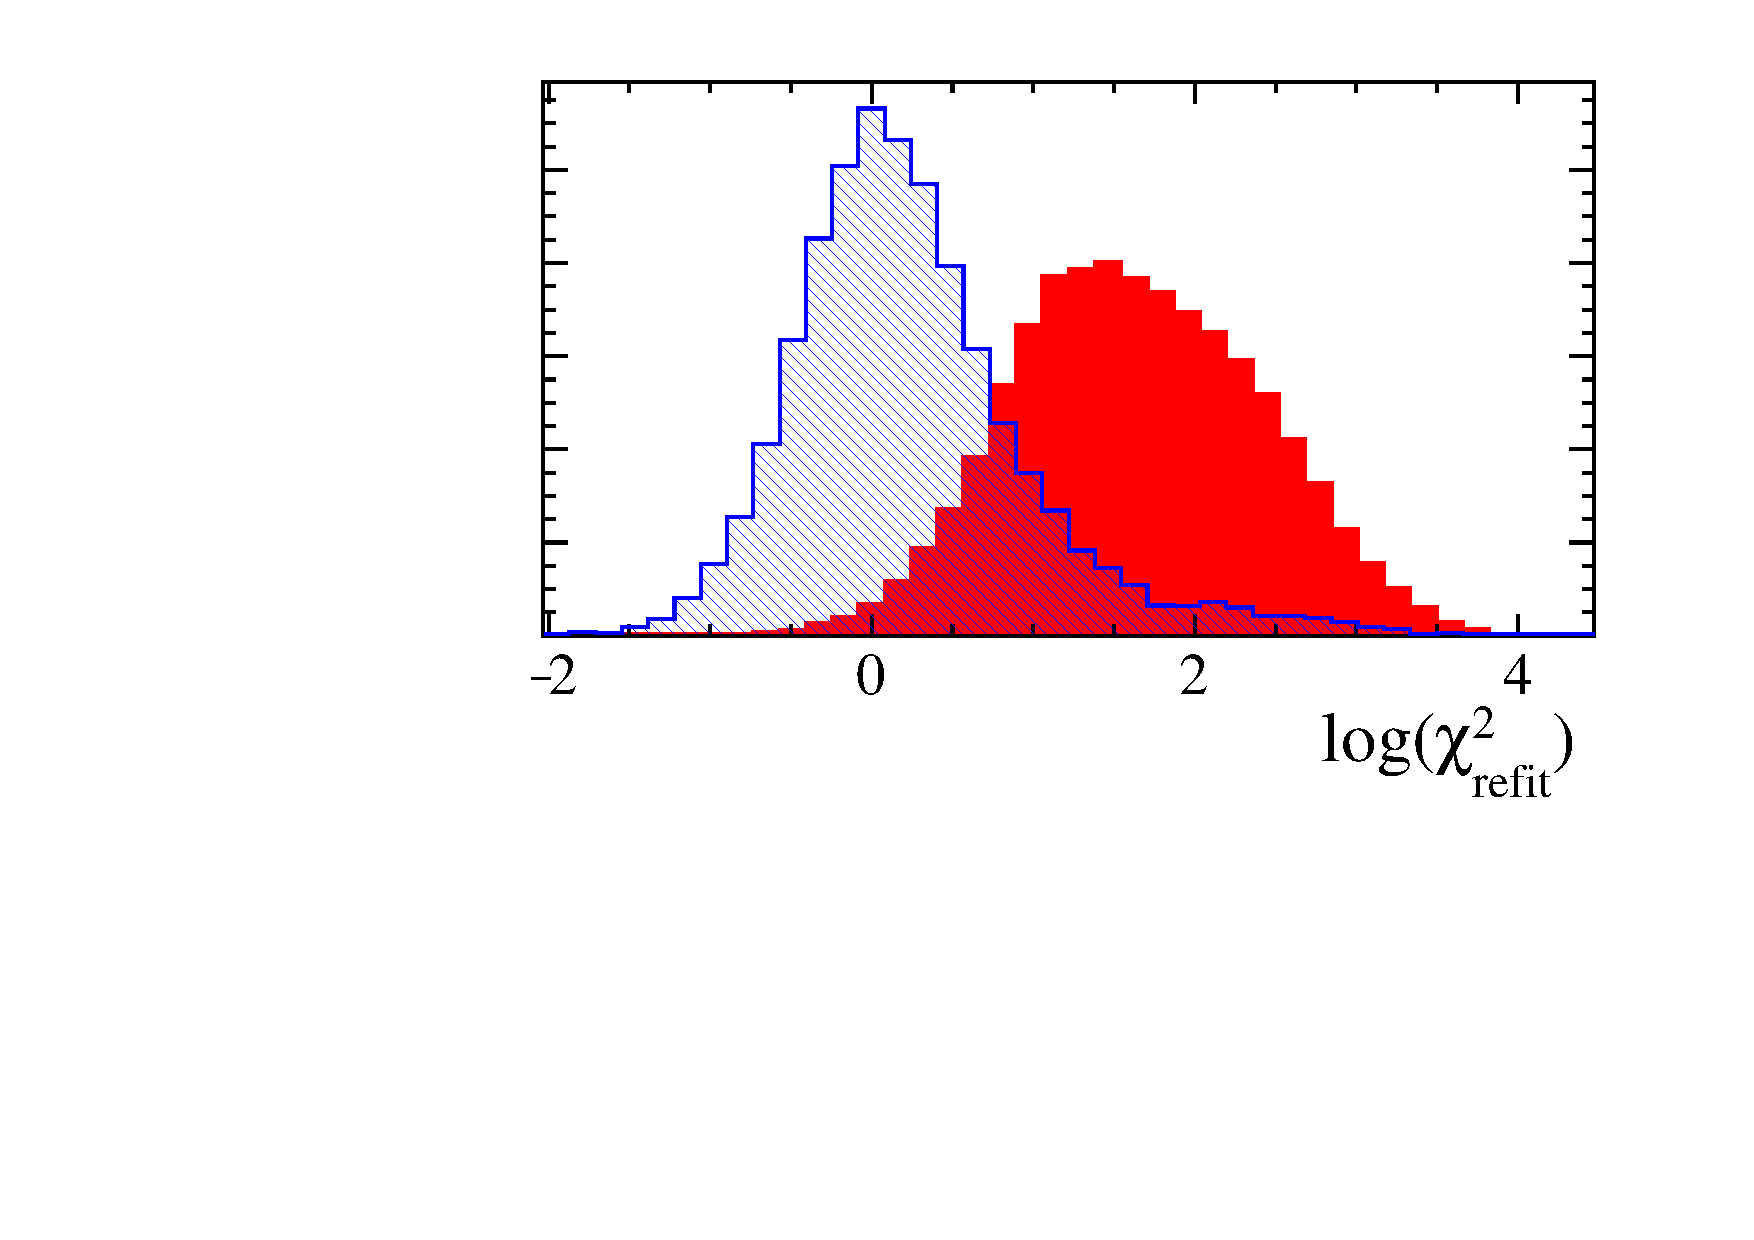
\includegraphics[width=0.3\linewidth]{figures/selection/BDTvariables/BDT_Var_KPiPiPi_DD_log_Bu_D0constKS0constPVconst_CHI2NDOF_.pdf}
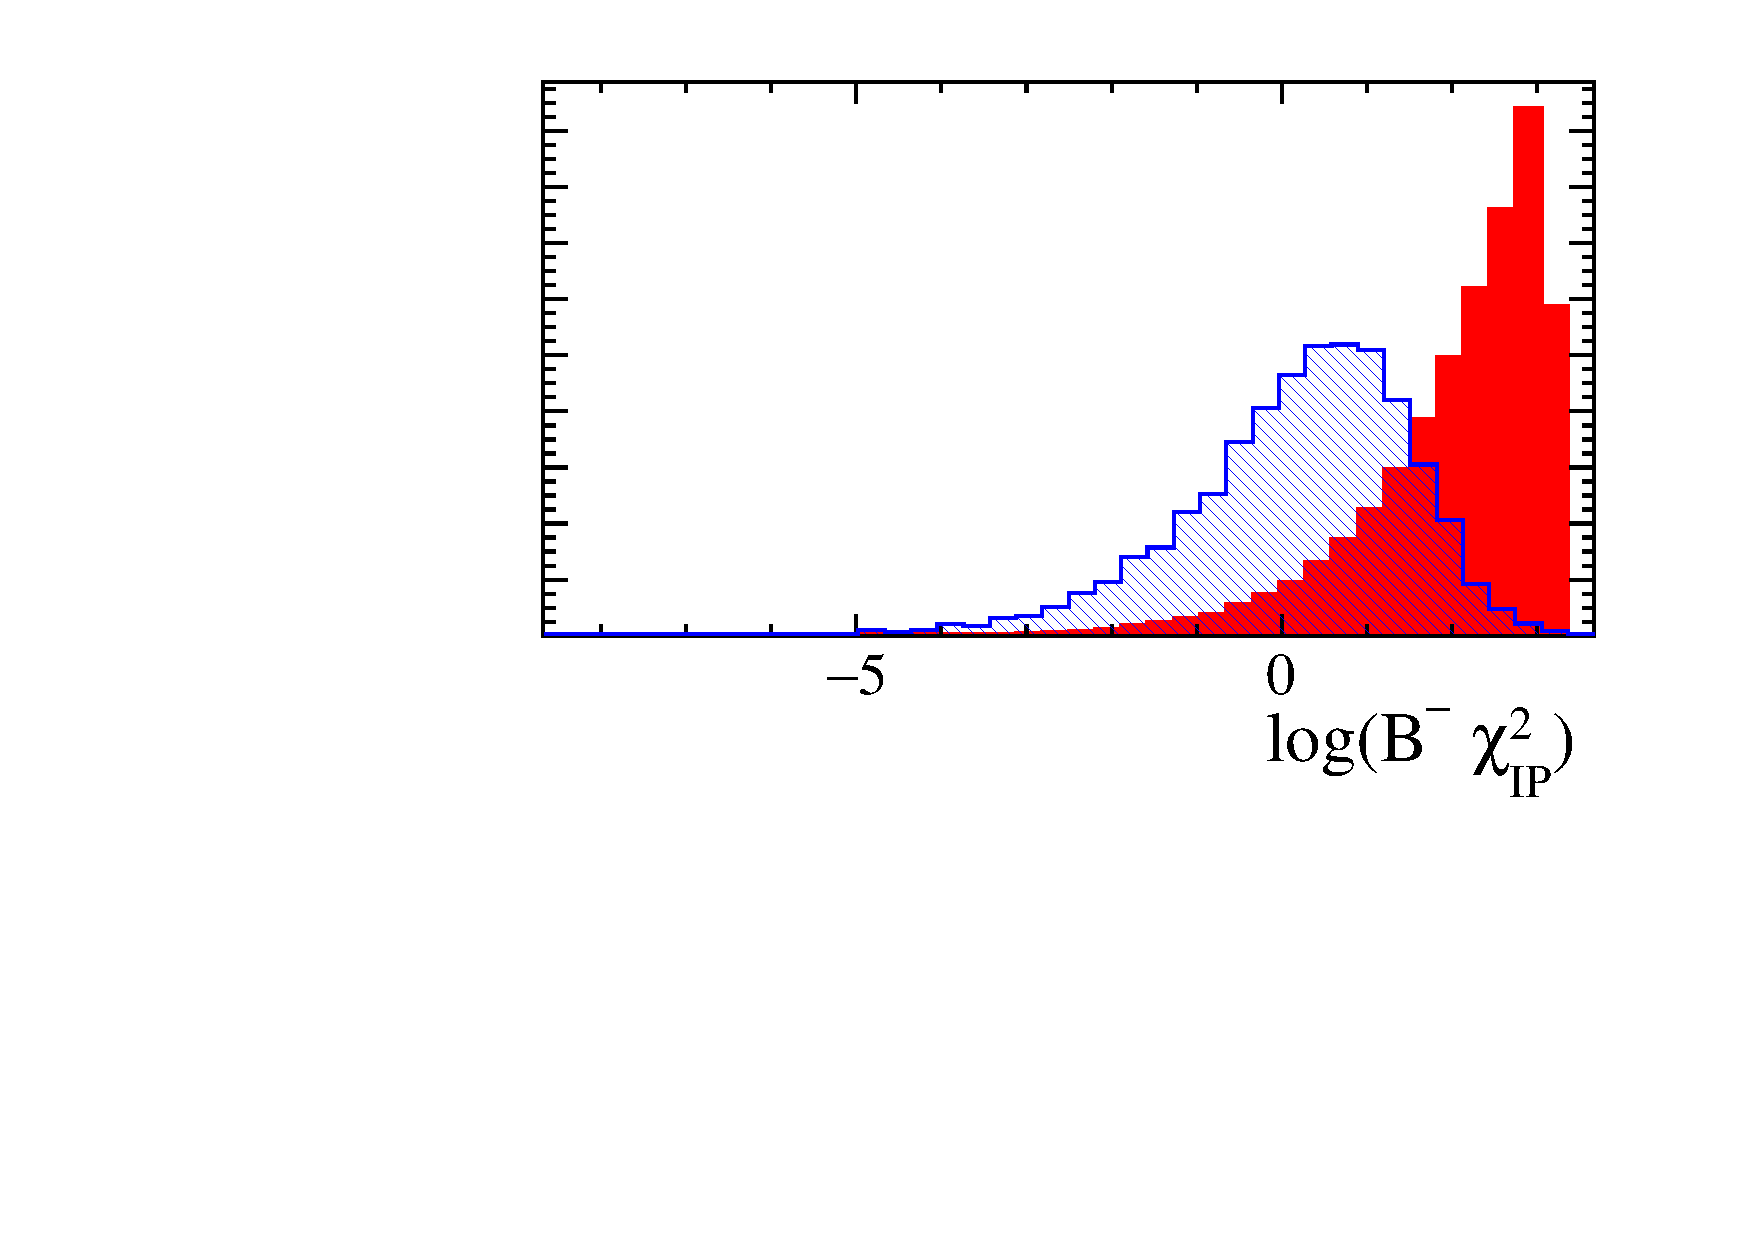
\includegraphics[width=0.3\linewidth]{figures/selection/BDTvariables/BDT_Var_KPiPiPi_DD_log_Bu_IPCHI2_OWNPV_.pdf}
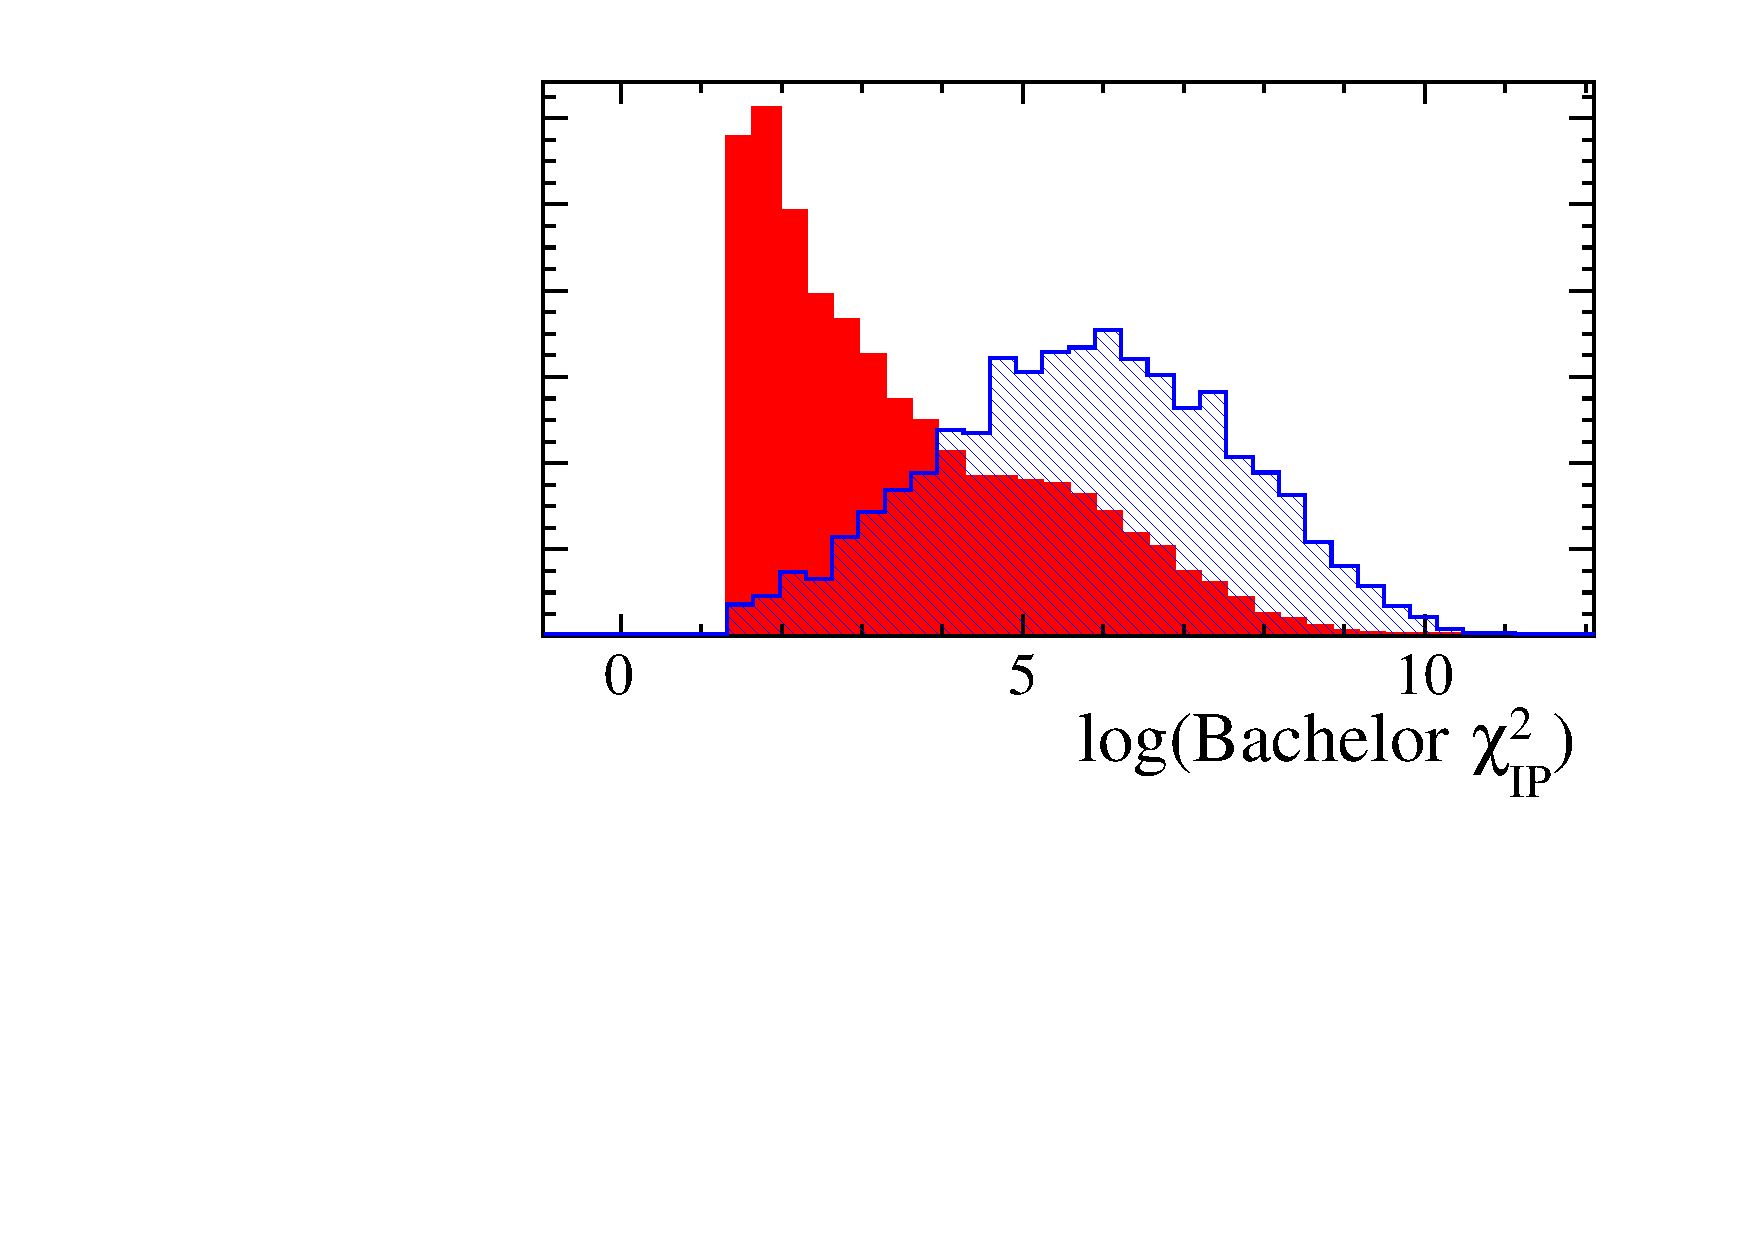
\includegraphics[width=0.3\linewidth]{figures/selection/BDTvariables/BDT_Var_KPiPiPi_DD_log_Bach_IPCHI2_OWNPV_.pdf}
\hfill
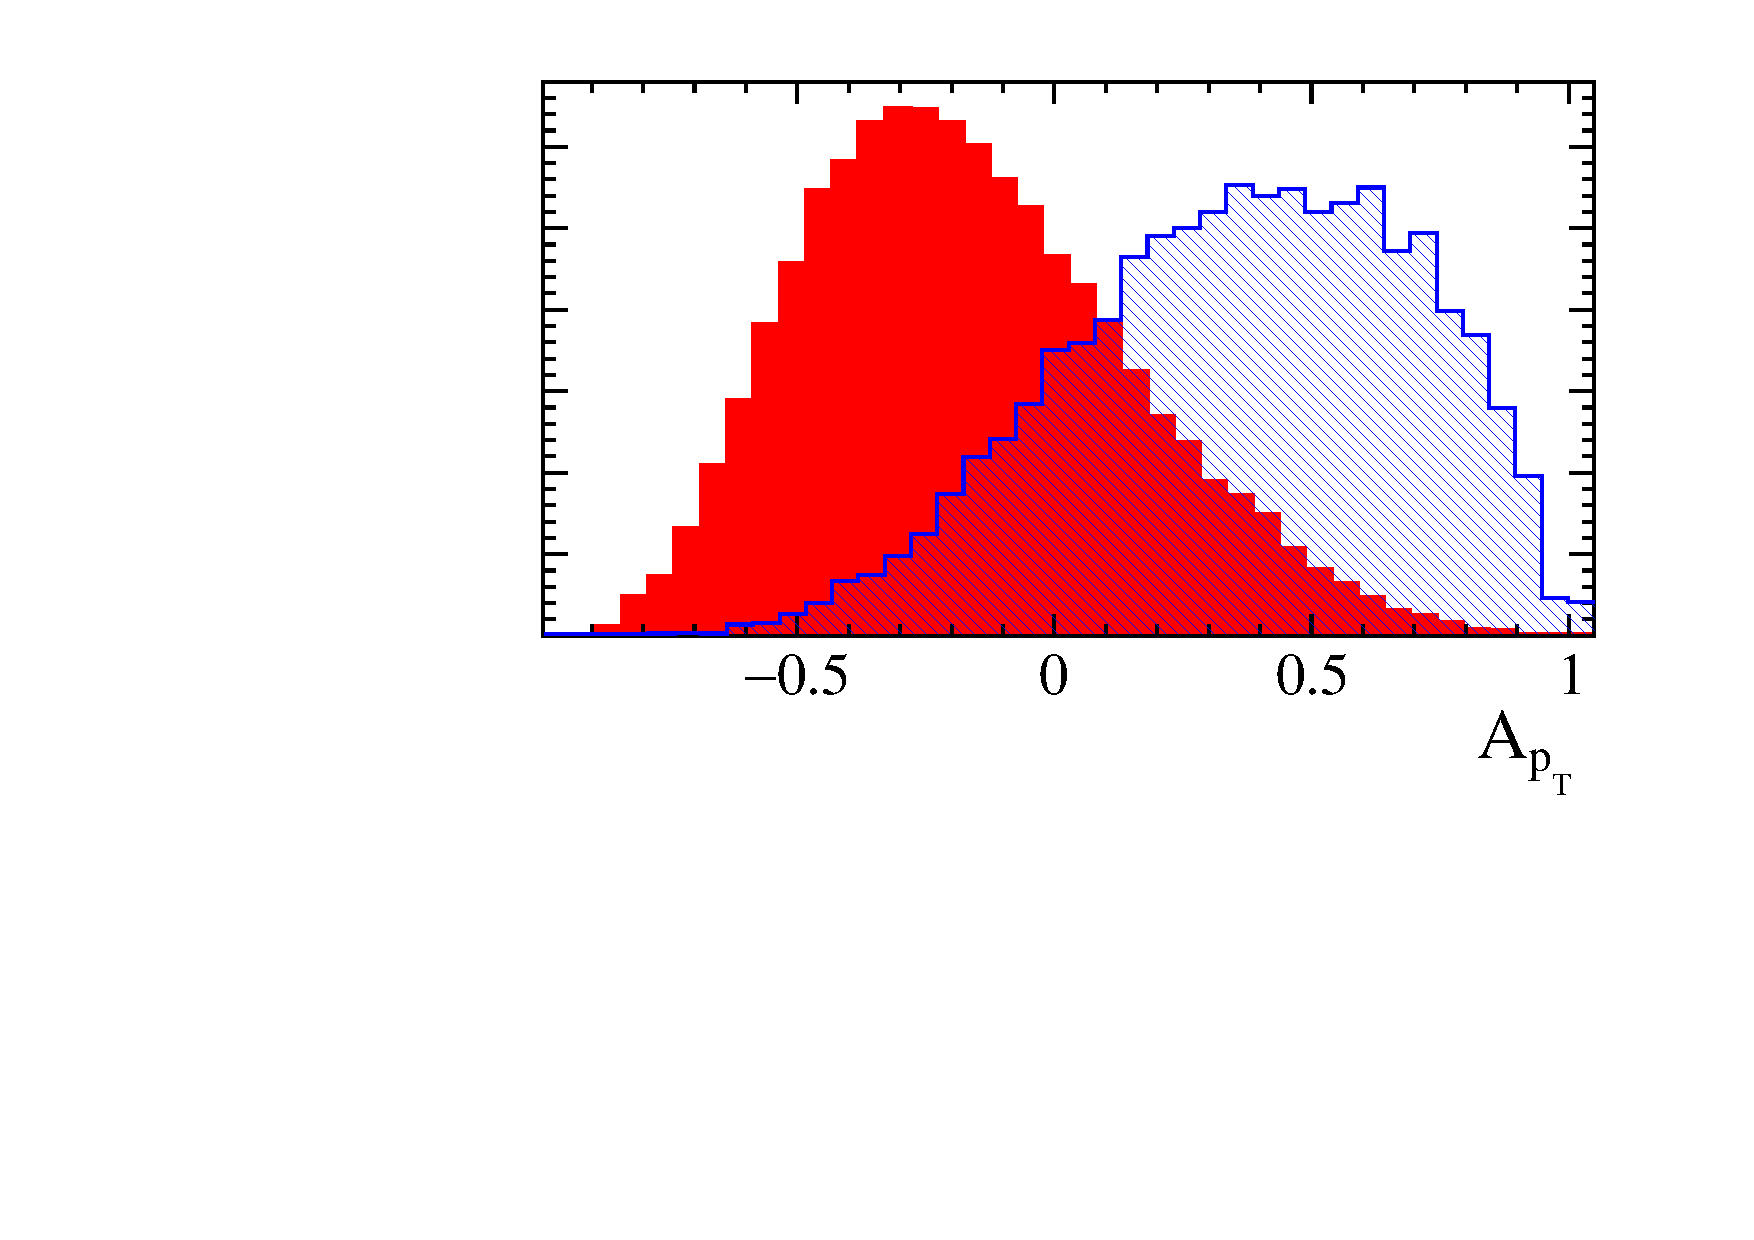
\includegraphics[width=0.3\linewidth]{{figures/selection/BDTvariables/BDT_Var_KPiPiPi_DD_Bu_ptasy_1.50}.pdf}
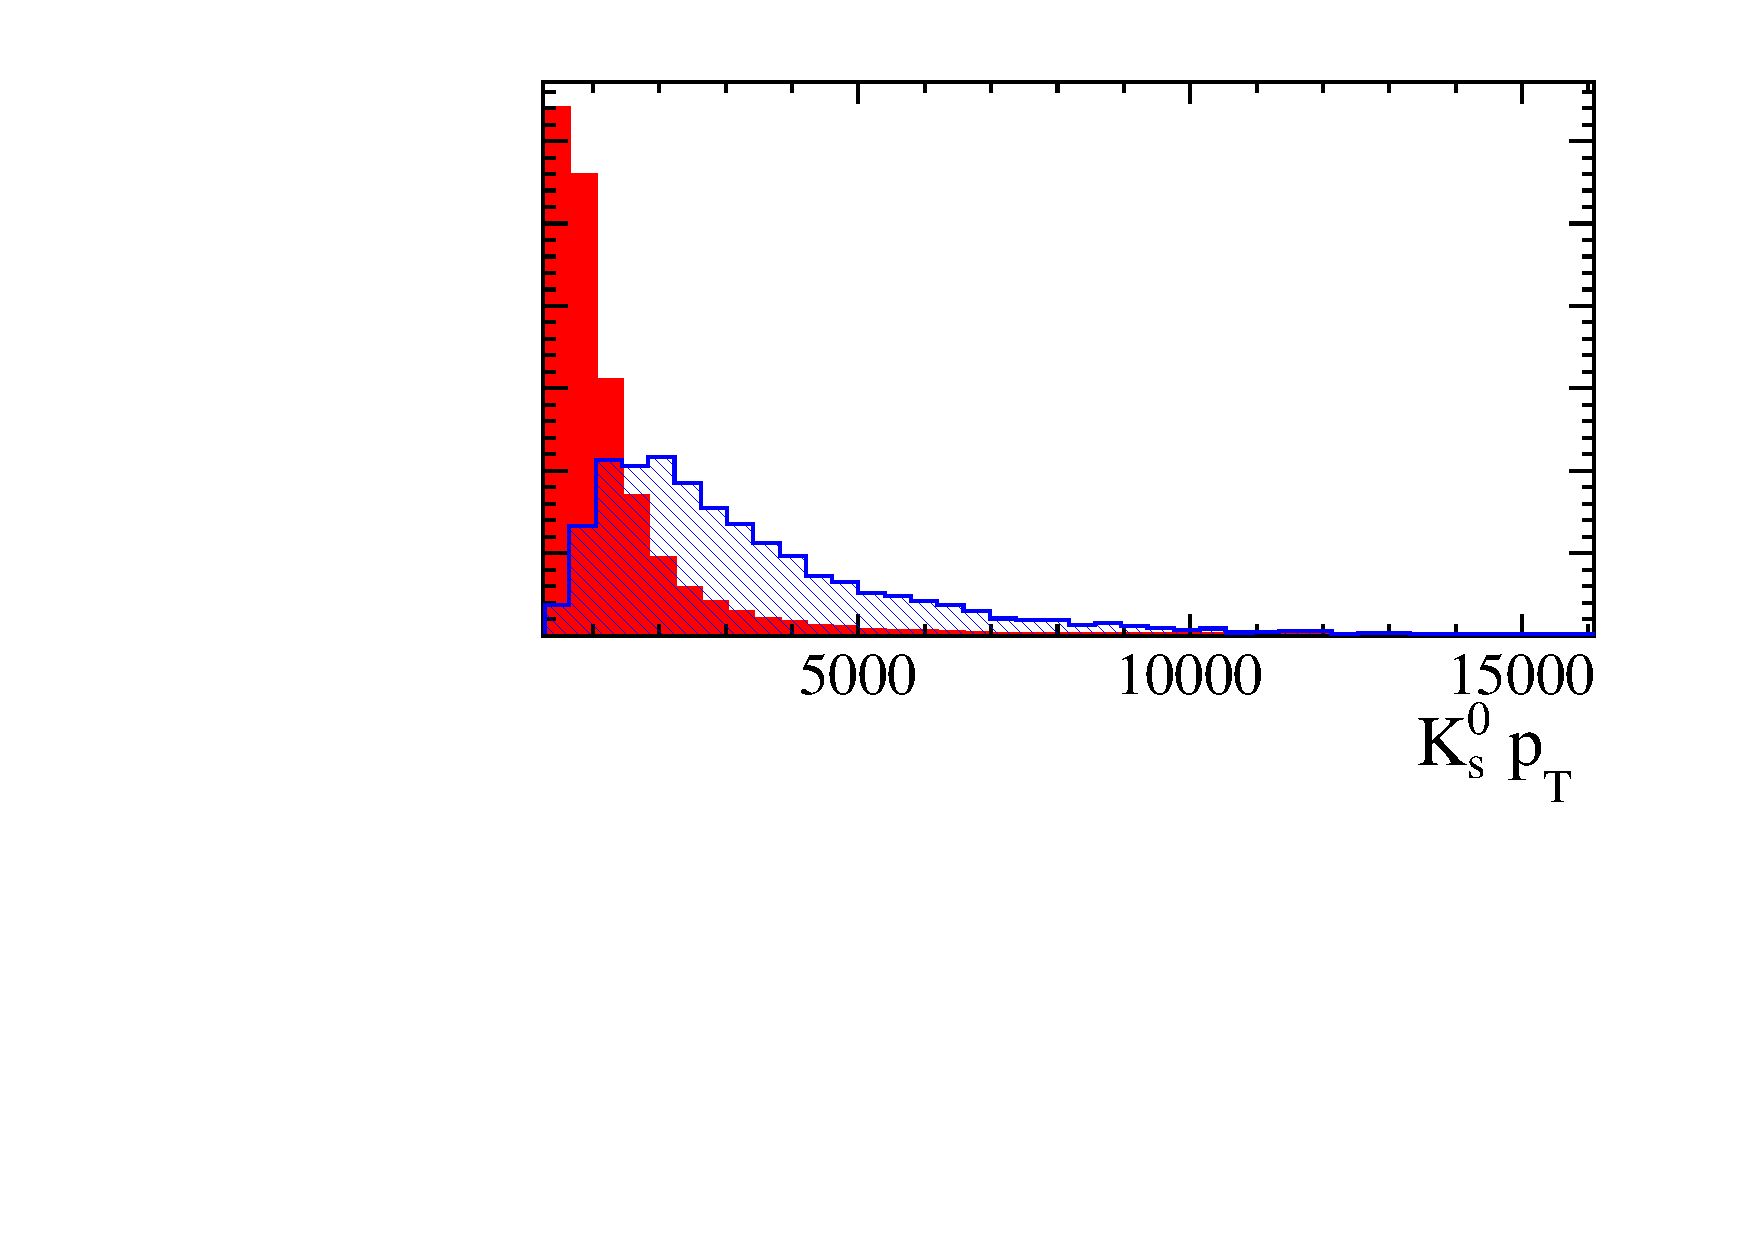
\includegraphics[width=0.3\linewidth]{figures/selection/BDTvariables/BDT_Var_KPiPiPi_DD_Ks_PT.pdf}
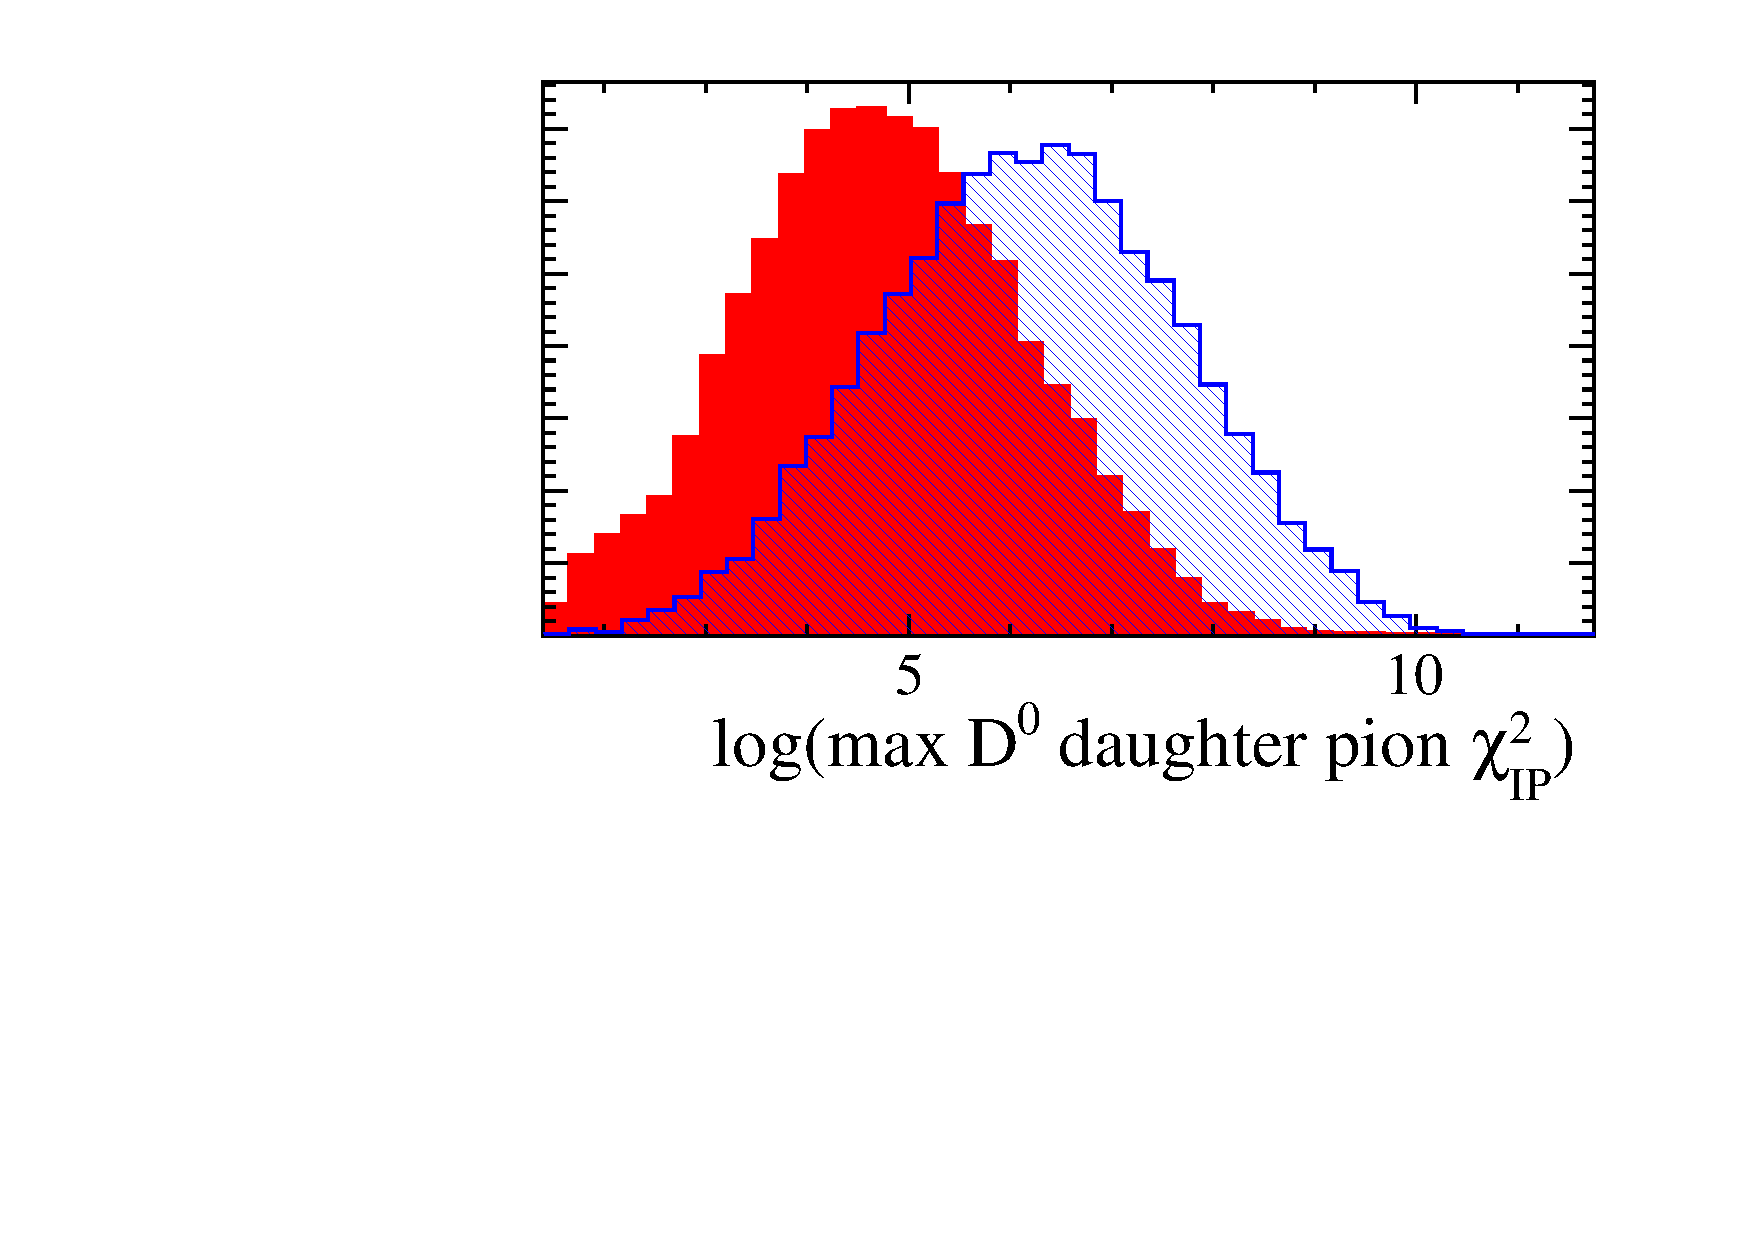
\includegraphics[width=0.3\linewidth]{figures/selection/BDTvariables/BDT_Var_KPiPiPi_DD_log_max_Dh_IPCHI2_OWNPV_.pdf}
\hfill
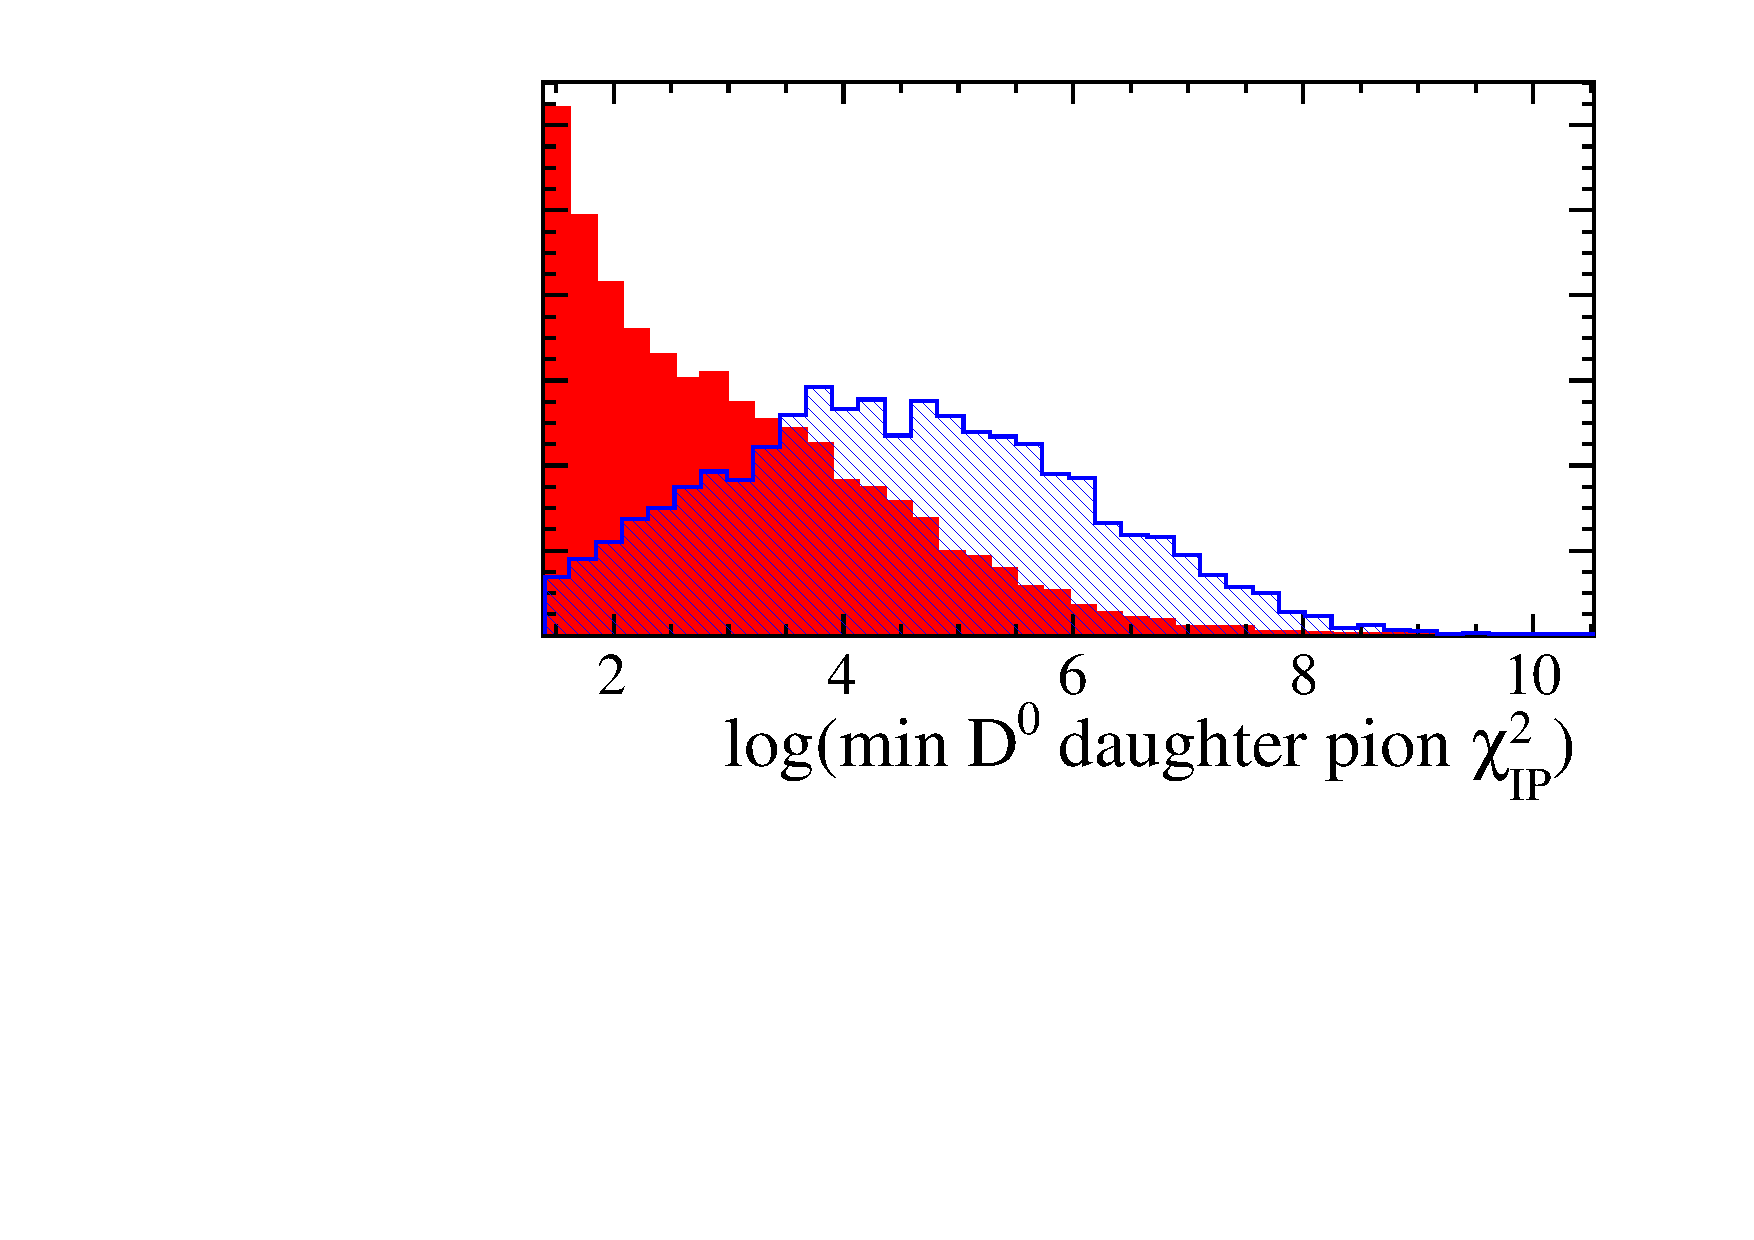
\includegraphics[width=0.3\linewidth]{figures/selection/BDTvariables/BDT_Var_KPiPiPi_LL_log_min_Dh_IPCHI2_OWNPV_.pdf}
\caption{Distributions of the input variables using the signal (blue) and background (red) training samples for the four-body DD BDT. The variable $A_{\pt}$ represents the \pt asymmetry as defined in \eqn~\ref{ptasy}. The particle name ``D daughter ss'' refers to the pion from the \Dz meson which has the same sign as the kaon. All distributions have been normalised to unity in order to easily compare their shape, therefore the vertical axis is not labelled as it is not of interest here.}
\label{BDTinputdist4bodyDD}
\end{figure}

\clearpage
